\chapter{反三角函数与简单三角方程的解法}
\section{反正弦函数}
我们知道,正弦函数$y=\sin x$是一个周期等于$2\uppi$的振动函
数,它的定义域是$(-\infty,+\infty)$, 而值域是闭区间$[-1,1]$, 它的图象如图9.1。

\begin{figure}[htp]
    \centering
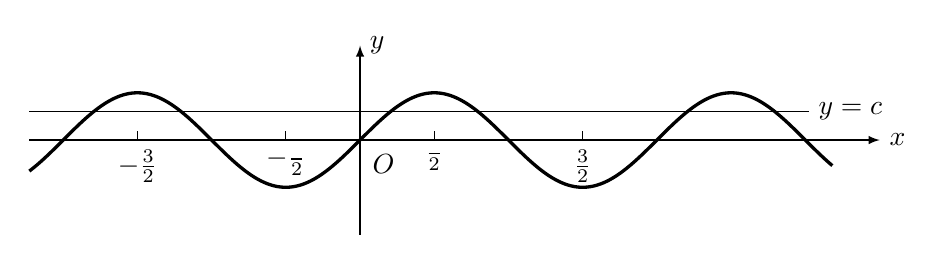
\begin{tikzpicture}[>=latex, scale=.6]
\draw[->] (-7,0)--(11,0)node[right]{$x$};
\draw [->] (0,-2)--(0,2)node[right]{$y$};

\draw[domain=-7:10, samples=1000, very thick] plot(\x,{sin(\x r)});
\draw  (-7,.6)--(9.5,0.6)node[right]{$y=c$};

\foreach \x/\xtext in {-1.5*pi/-\frac{3\uppi}{2}, -.5*pi/-\frac{\uppi}{2},.5*pi/\frac{\uppi}{2}, 1.5*pi/\frac{3\uppi}{2}}
{
    \draw (\x,0)node[below]{$\xtext$}--(\x,.2);
}
\node at (.5,-.5){$O$};
\end{tikzpicture}
    \caption{}
\end{figure}


每取一数$y=c,\; -1\leqslant c\leqslant 1$, 作直线$y=c$, 可与正弦曲线
$y=\sin x$交于无穷多个点,这些交点的横坐标是
\[x=x_0+2k\uppi\qquad \text{和}\qquad x=(\uppi -x_0)+2k\uppi\quad (k\in\mathbb{Z})\]
因此有无数多个$x$的值满足方程$\sin x =c$, 而和那个$y=c$对
应。可见对于变数$x$的一切可能实数值来说,我们不能由函
数$f:\mathbb{R}\to [-1,1]$, $f(x)=\sin x$得出它的反函数来。把定
义域分成无数个单调区间,则在各区间$\left[-\frac{\uppi}{2}+2k\uppi, \frac{\uppi}{2}+2k\uppi\right]$上,$y=\sin x$由$-1$上升到1,而在各区间$\left[\frac{\uppi}{2}+2k\uppi, \frac{3\uppi}{2}+2k\uppi\right]$上,$y=\sin x$由1下降到$-1$,于是由前一章中的
反函数定理知道,对于上述每一个单调区间存在一个反函数。

如果我们强调的是在闭区间$\left[-\frac{\uppi}{2},\frac{\uppi}{2}\right]$上
来考虑正弦
函数的反函数,我们就说它是反正弦函数的主值,并把这个函数记作
$x=\arcsin y$,使得
$$x=\arcsin y\qquad \Longleftrightarrow \qquad y=\sin x$$
这里$x\in \left[-\frac{\uppi}{2},\frac{\uppi}{2}\right],\quad y\in[-1,+1]$。

对于使得$y=\sin x$是单调的另一区间,例如$x\in \left[\frac{\uppi}{2},\frac{3\uppi}{2}\right]$,
我们就得到另一个反正弦函数。假如我们没有明确地指出反正弦函数的值域所在的区间,我们就不能由函数 $y=\sin x$ 得出它的反函数。为了明确起见,现在我们规定

\begin{Definition}%{定义1}
函数 $y=\sin x$ 在闭区间 $\left[-\frac{\uppi}{2},\frac{\uppi}{2}\right]$ 上
的反函数叫做\emph{反正弦函数}或\emph{反正弦},这个函数用记号写作
$x=\arcsin y$ (即$x$是一角或弧,其相应的正弦值为$y$),
它的定义域是闭区间$-1\leqslant y\leqslant 1$, 值域是闭区间$-\frac{\uppi}{2}\leqslant x\leqslant \frac{\uppi}{2}$。
\end{Definition}

用习惯上的写法,将字母 $x$ 与 $y$ 互换而写成 $y=\arcsin x$,
现在,我们将反正弦函数(主值)的定义用几何名词叙述如下:

在闭区间 $-1\leqslant x\leqslant 1$ 上,数 $x$ 的反正弦 $y=\arcsin x$ 是在
闭区间 $\left[-\frac{\uppi}{2},\frac{\uppi}{2}\right]$ 上的一个角或弧,它的正弦值等于 $x$,即 $\sin y=x$。

由反正弦函数的定义和前一章的反函数定理可得到
它的一些性质如下:
\begin{itemize}
    \item $\arcsin(\sin y)=y,\qquad -\frac{\uppi}{2}\leqslant y\leqslant \frac{\uppi}{2}$
    
    $\sin(\arcsin x)=x,\qquad -1\leqslant x\leqslant 1$

    \item 函数$f(x)=\arcsin x$在闭区间$[-1,1]$上单调递
    增,并且连续。
    \item $y=\arcsin x,\; -1\leqslant x\leqslant 1$的图象与$y=\sin x,\; -\frac{\uppi}{2}\leqslant y\leqslant \frac{\uppi}{2}$
    的图象关于直线$y=x$对称(图5.2)。
\end{itemize}

\begin{figure}[htp]
    \centering
\begin{tikzpicture}[>=latex, scale=1]
\draw[->] (-4,0)--(4,0)node[right]{$x$};
\draw [->] (0,-3)--(0,3)node[right]{$y$};

\draw[domain=-pi:pi, samples=1000, dashed, thick] plot(\x,{sin(\x r)});
\draw[domain=-1:1, samples=1000, very thick] plot(\x,{asin(\x)*pi/180});
\draw[dashed] (-3,-3)--(2.5,2.5)node [above]{$y=x$};
\draw [dashed] (0,.5*pi)node[left]{$\frac{\uppi}{2}$}--(1,.5*pi)node[above]{$y=\arcsin x$};
\draw [dashed] (0,-.5*pi)node[right]{$-\frac{\uppi}{2}$}--(-1,-.5*pi);
\node at (.25,-.25){$O$};
\node at (pi+.5,0)[above]{$y=\sin x$};
\foreach \x in {-1,1}
{
    \draw (\x,0)node[below]{$\x$}--(\x,.1);
}
\draw (0,1)node[left]{$1$}--(.1,1);
\draw (0,-1)--(-.1,-1)node[right]{$-1$};

\end{tikzpicture}
    \caption{}
\end{figure}



我们已知正弦函数是奇函数,它的图象关于原点对称,
现在我们要证明 $f(x)=\arcsin x$是奇函数,即
$\arcsin(-x)=-\arcsin x$。

\begin{proof}
    因为$-\frac{\uppi}{2}\leqslant \arcsin x\leqslant \frac{\uppi}{2}$,
    角$-\arcsin x$也被限制在由$-\frac{\uppi}{2}$到$\frac{\uppi}{2}$
    的区间内:
    $$-\frac{\uppi}{2}\leqslant -\arcsin x\leqslant \frac{\uppi}{2}$$
    又,角$-\arcsin x$的正弦等于$-x$
\[\sin(-\arcsin x)=-\sin(\arcsin x)=-x\]
因此:$\arcsin(-x)=-\arcsin x$。
\end{proof}

\begin{example}
    求下列各式的值(口答):
    \begin{enumerate}
        \item $\arcsin\frac{1}{2}$
        \item $\arcsin\left(-\frac{1}{2}\right)$
        \item $\arcsin 1$
    \end{enumerate}
\end{example}

\begin{solution}
\begin{enumerate}
    \item $\arcsin\frac{1}{2}=\frac{\uppi}{6}$,因为$\sin\frac{\uppi}{6}=\frac{1}{2}$,且$-\frac{\uppi}{2}<\frac{\uppi}{6}<\frac{\uppi}{2}$

    \item $\arcsin\left(-\frac{1}{2}\right)=-\frac{\uppi}{6}$,因为$\sin\left(-\frac{\uppi}{6}\right)=-\frac{1}{2}$,且
    $-\frac{\uppi}{2}<-\frac{\uppi}{6}<\frac{\uppi}{2}$
    \item $\arcsin 1=\frac{\uppi}{2}$,因为$\sin\frac{\uppi}{2}=1$,而且$\frac{\uppi}{2}$不超出$\left[-\frac{\uppi}{2},\frac{\uppi}{2}\right]$的界限。
\end{enumerate}
\end{solution}

\begin{example}
    求下列各式的值:
\[\arcsin\left(-\frac{\sqrt{3}}{2}\right),\qquad \arcsin (-0.2672) \]
\end{example}

\begin{solution}
\begin{enumerate}
    \item $\arcsin\left(-\frac{\sqrt{3}}{2}\right)=-\arcsin\frac{\sqrt{3}}{2}=-\frac{\uppi}{3}$
    \item $\arcsin(-0.2672)=-\arcsin0.2672=-15^{\circ}30'\approx -0.2705$
\end{enumerate}
    
\end{solution}



\begin{example}
    求下列各式的值:
\begin{tasks}(2)
  \task $\sin\left(\arcsin\frac{1}{3}\right)$
  \task $\tan\left(\arcsin\frac{\sqrt{2}}{2}\right)$
  \task $\cos\left(\arcsin\frac{3}{5}\right)$
  \task $\sin\left[2\arcsin\left(-\frac{3}{5}\right)\right]$
  \task $\arcsin\left(\sin\frac{7\uppi}{6}\right)$
\end{tasks}
\end{example}

\begin{solution}
\begin{enumerate}
    \item $\sin\left(\arcsin\frac{1}{3}\right)=\frac{1}{3}$
    \item $\tan\left(\arcsin\frac{\sqrt{2}}{2}\right)=\tan\frac{\uppi}{4}=1$
    \item 设$\arcsin\frac{3}{5}=\alpha$,其中$-\frac{\uppi}{2}\le\alpha\le\frac{\uppi}{2}$,那么$\sin\alpha=\frac{3}{5}$。由于$-\frac{\uppi}{2}\le\alpha\le\frac{\uppi}{2}$,$\sin\alpha>0$,可以知道,$\alpha$是第一象限的角,所以
    $$\cos\left(\arcsin\frac{3}{5}\right)=\sqrt{1-\left(\frac{3}{5}\right)^2}=\frac{4}{5}$$
    \item 设$\arcsin\left(-\frac{3}{5}\right)=\alpha$,其中$-\frac{\uppi}{2}\le\alpha\le\frac{\uppi}{2}$,那么
    \[\sin\alpha =\sin\left[\arcsin\left(-\frac{3}{5}\right)\right]=-\frac{3}{5}\]
由于$-\frac{\uppi}{2}\le\alpha\le\frac{\uppi}{2}$和$\sin\alpha<0$,可以知道$\alpha$是第四象限的角,所以
\[\cos\alpha=\sqrt{1-\left(-\frac{3}{5}\right)^2}=\frac{4}{5}\]
即:
$\sin\left[2\arcsin\left(-\frac{3}{5}\right)\right]=\sin2\alpha=2\sin\alpha\cdot \cos\alpha=2\left(-\frac{3}{5}\right)\cdot\left(\frac{4}{5}\right)=-\frac{24}{25}$
    \item \[\begin{split}
\arcsin\left(\sin\frac{7\uppi}{6}\right)&=\arcsin\left[\sin\left(\uppi+\frac{\uppi}{6}\right)\right]\\
&=\arcsin\left(-\sin\frac{\uppi}{6}\right)\\
&=-\arcsin\left(\sin\frac{\uppi}{6}\right)=-\frac{\uppi}{6}        
    \end{split}\]
\end{enumerate}
\end{solution}

关于 $y=\sin x$, 只要知道了它在闭区间 $-\frac{\uppi}{2}\leqslant x\leqslant \frac{\uppi}{2}$ 上
的反函数 $x=\arcsin y$,我们便能求出 $y=\sin x$ 在其它单调区间上的反函数。

\begin{Theorem}{命题}
\begin{enumerate}
    \item $y=\sin x$在闭区间$\left[-\frac{\uppi}{2}+2k\uppi,\frac{\uppi}{2}+2k\uppi\right]$上,由$-1$上升到1,它们相应的反函数是
\[x=\arcsin y+2k\uppi,\quad k\in\mathbb{Z}\]
因为
\[\sin x= \sin(\arcsin y+ 2k\uppi) = \sin(\arcsin y) = y\]
而且
\[-\frac{\uppi}{2}+2k\uppi\leqslant \arcsin y+2k\uppi \leqslant \frac{\uppi}{2}+2k\uppi
,\quad k\in\mathbb{Z}\]
    
\item\label{itm:arcsin_case2} $y=\sin x$在闭区间$\left[\frac{\uppi}{2},\frac{3\uppi}{2}\right]$上,由1下降到$-1$,
它的反函数是
\[x=\uppi-\arcsin y\]
因为
\[\sin x=\sin(\uppi- \arcsin y) = \sin(\arcsin y) = y\]
而且
\[\frac{\uppi}{2}=\uppi-\frac{\uppi}{2} \leqslant \uppi-\arcsin y \leqslant \uppi+\frac{\uppi}{2}=\frac{3\uppi}{2}\]
我们也可以在单位圆上作图来说明 \ref{itm:arcsin_case2},如图9.3所示。

\item $y=\sin x$ 在闭区间 $\left[\dfrac{\uppi}{2}+2k\uppi,\dfrac{3\uppi}{2}+2k\uppi\right]$上,由
1下降到$-1$, 相仿地证得它在相应区间上的反函数是
\[x=(\uppi-\arcsin y)+2k\uppi,\quad k\in\mathbb{Z} \]
\end{enumerate}
\end{Theorem}

\begin{figure}[htp]
    \centering
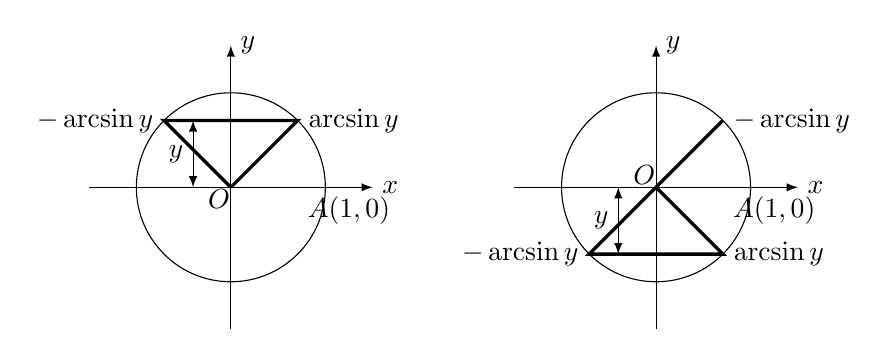
\begin{tikzpicture}[>=latex, scale=.6]
\begin{scope}
    \draw[->] (-3,0)--(3,0)node[right]{$x$};
    \draw[->] (0,-3)--(0,3)node[right]{$y$};
    \draw (0,0) circle(2);
    \node at (-.25,-.25){$O$};
\node at (2.5,0)[below]{$A(1,0)$};
\draw[very thick] (0,0)--(45:2)node[right]{$\arcsin y$}--(90+45:2)node[left]{$\uppi-\arcsin y$}--(0,0);

\draw[<->] (-.8,0)--node[left]{$y$}(-.8,1.414);
\end{scope}

\begin{scope}[xshift=9cm]
    \draw[->] (-3,0)--(3,0)node[right]{$x$};
    \draw[->] (0,-3)--(0,3)node[right]{$y$};
    \draw (0,0) circle(2);
    \node at (-.25,.25){$O$};
\node at (2.5,0)[below]{$A(1,0)$};

\draw[<->] (-.8,0)--node[left]{$y$}(-.8,-1.414);
\draw[very thick] (0,0)--(-45:2)node[right]{$\arcsin y$}--(-90-45:2)node[left]{$\uppi-\arcsin y$}--(0,0);
\draw[very thick] (0,0)--(45:2)node[right]{$-\arcsin y$};
\end{scope}
\end{tikzpicture}

    \caption{}
\end{figure}


\begin{example}
  讨论函数 $y=\arcsin(\sin x)$ 的图象。
\end{example}

\begin{solution}
  由于正弦的周期性,函数 $\arcsin(\sin x),\; x\in\mathbb{R}$ 也以 $2\uppi$ 为周期,因此,只研究它在长度为 $2\uppi$ 的区间内情形即可。由于
  \[\sin y=\sin[\arcsin(\sin x)]=\sin x\]
  这里 $-\frac{\uppi}{2}\leqslant y\leqslant \frac{\uppi}{2}$,而 $x\in\mathbb{R}$,故
  \begin{itemize}
    \item 当 $x\in\left[-\frac{\uppi}{2},\frac{\uppi}{2}\right]$ 时,则 $y=x$。
    \item 当 $x\in\left[\frac{\uppi}{2},\frac{3\uppi}{2}\right]$ 时,则由上面的命题 2 知
    \[x=\uppi-y\quad \Rightarrow\quad y=\uppi-x\in \left(-\frac{\uppi}{2},\frac{\uppi}{2}\right)\]
  \end{itemize}
因之,在此区间内函数的图象与直线 $y=\uppi-x$ 一致,总之,由上面的命题中的 1 和 3 的结果:
\begin{enumerate}
  \item 当$x\in \left[-\frac{\uppi}{2}+2k\uppi,\frac{\uppi}{2}+2k\uppi\right]$时,则$x=y+2k\uppi$,则$y=x-2k\uppi$;
  \item 当$x\in \left[\frac{\uppi}{2}+2k\uppi,\frac{3\uppi}{2}+2k\uppi\right]$时,则$x=\uppi-y+2k\uppi$,则$y=(\uppi-x)-2k\uppi$。
\end{enumerate}
由上面讨论的结果,得到函数 $y= \arcsin(\sin x)$ 的图象是折线的形状,如图 5.4所示。
\begin{figure}[htp]
    \centering
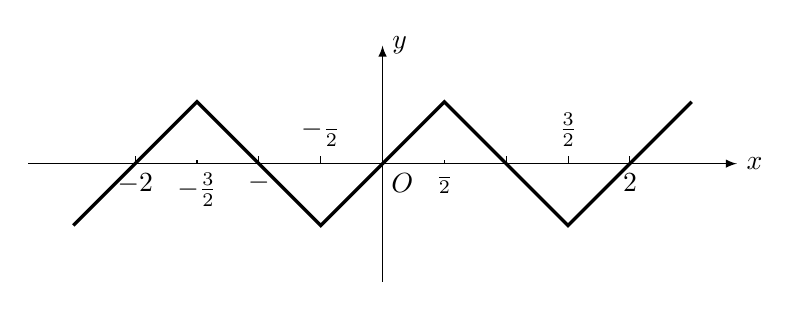
\begin{tikzpicture}[>=latex, scale=.5]
    \draw[->] (-9,0)--(9,0)node[right]{$x$};
    \draw[->] (0,-3)--(0,3)node[right]{$y$};
\draw[very thick] (-2.5*pi,-0.5*pi)--(-1.5*pi,.5*pi)--(-.5*pi,-0.5*pi)--(.5*pi,.5*pi)--(1.5*pi,-0.5*pi)--(2.5*pi,.5*pi);
\foreach \x/\xtext in {-2/-2\uppi, -1/-\uppi,1/\uppi,2/2\uppi}
{
    \draw (pi*\x,0)node[below]{$\xtext$}--(pi*\x,0.2);
}
\foreach \x/\xtext in {.5/\frac{\uppi}{2},-1.5/-\frac{3\uppi}{2}}
{
    \draw (pi*\x,0)node[below]{$\xtext$}--(pi*\x,0.1);
}
\foreach \x/\xtext in {1.5/\frac{3\uppi}{2},-.5/-\frac{\uppi}{2}}
{
    \draw (pi*\x,0)--(pi*\x,0.2)node[above]{$\xtext$};
}
\node at (.5,-.5){$O$};

\end{tikzpicture}
    \caption{}
\end{figure}
\end{solution}


\begin{Exercise}
\begin{question}
    \item 用反三角函数表示下面等式中的角。
\begin{tasks}(2)
    \task $\sin\frac{\uppi}{4}=\frac{\sqrt{2}}{2}$
    \task $\sin\frac{5\uppi}{3}=-\frac{\sqrt{3}}{3}$
    \task $\sin\frac{7\uppi}{3}=\frac{\sqrt{3}}{2}$
    \task $\sin(-2.314)=-0.04038$
\end{tasks}
    \item 当$\frac{1}{2}\leqslant x\le\frac{\sqrt{3}}{2}$
    时,求函数$y=x\arcsin x$的最大值
    和最小值。
    \item 不求值,确定下面差的符号:
\begin{tasks}
    \task $\arcsin 0.7-\arcsin 0.5$
    \task $\arcsin\left(-\frac{3}{5}\right)-\arcsin\left(-\frac{3}{4}\right)$
    \task $\arcsin\left(\sqrt{2}-1\right)-\arcsin\left(\sqrt{5}-2\right)$
\end{tasks}
\item 求下列各式的值:
\begin{tasks}(2)
    \task $\arcsin\frac{\sqrt{3}}{2}$
    \task $\arcsin\left(-\frac{\sqrt{2}}{2}\right)$
    \task $\arcsin0$
    \task $\arcsin(-1)$
    \task $\arcsin\left(-\frac{1}{4}\right)$
    \task $\arcsin0.7841$
\end{tasks}

\item 计算下列各式的值:
    \begin{tasks}(2)
        \task $\tan\left(\arcsin\frac{\sqrt{2}}{2}\right)$
        \task $\cos\left(\arcsin \frac{3}{5}\right)$
        \task $\arcsin \left[\sin\left(-\frac{\uppi}{7}\right)\right]$
        \task $\arcsin\left(\sin\frac{5\uppi}{6}\right)$
        \task $\arcsin(\cos1)$
    \end{tasks}
    \item 计算下列各式的值:
    \begin{tasks}(2)
        \task $\cot\left(2\arcsin\frac{\sqrt{2}}{2}\right)$
        \task $\cos\left(2\arcsin\frac{1}{3}\right)$
        \task $\sin\left(3\arcsin\left(-\frac{\sqrt{3}}{2}\right)\right)$
        \task $\tan\left(\frac{1}{2}\arcsin\frac{2}{3}\right)$
    \end{tasks}

    \item 讨论函数$y=x \arcsin(\sin x)$的图象,并作草图。
\item 画出$f(x)=\sin(3\arcsin x)$的图象。
\end{question}
\end{Exercise}

\section{反余弦函数}
由余弦函数$y=\cos x$的图象(图9.5)看出,函数$y=\cos x$
在闭区间$[2k\uppi ,(2k+1)\uppi ]$上,由1下降到$-1$, 而在闭区间
$[(2k-1)\uppi ,2k\uppi]$上,由$-1$上升到1; 因此,对于上述每一
个单调区间,函数$y=\cos x$都带来一个反函数。

\begin{figure}[htp]
    \centering
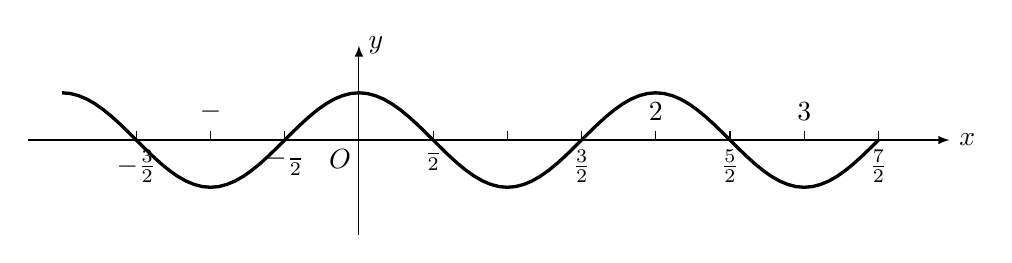
\begin{tikzpicture}[>=latex, scale=.6]
\draw[->] (-7,0)--(12.5,0)node[right]{$x$};
\draw[->] (0,-2)--(0,2)node[right]{$y$};
\foreach \x/\xtext in {-3/-\frac{3\uppi}{2},-1/-\frac{\uppi}{2},1/\frac{\uppi}{2},3/\frac{3\uppi}{2},5/\frac{5\uppi}{2},7/\frac{7\uppi}{2}}
{
    \draw(\x*pi/2, 0)node[below]{$\xtext$}--(\x*pi/2,.2);
}
\foreach \x/\xtext in {-1/-\uppi, 1/\uppi, 2/2\uppi, 3/3\uppi}
{
    \draw(\x*pi, 0)--(\x*pi,.2)node[above]{$\xtext$};
}
\draw [domain=-2*pi:3.5*pi, samples=100, very thick]plot(\x, {cos(\x r)});
\node at (-.4,-.4){$O$};
\end{tikzpicture}
    \caption{}
\end{figure}

\begin{Definition}
    函数$y=\cos x$在闭区间$[0,\uppi]$上的反函数叫做\emph{反
余弦函数}或\emph{反余弦},记作
\[x=\arccos y\]
它的定义域是闭区间$[-1,1]$。
\end{Definition}

用几何名词来叙述这个定义,便是(互换字母$x$、$y$的
位置):在闭区间$-1\leqslant x\leqslant 1$上,数$x$的反余弦
$y=\arccos x$
是在闭区间$[0,\uppi]$的一个角或弧,它的余弦值等于$x$, 即
$\cos y=x$。

\begin{example}
    求下列各式的值(口答):
\begin{tasks}(2)
    \task $\arccos\frac{1}{2}$
    \task $\arccos\left(-\frac{1}{2}\right)$
    \task $\arccos1$
    \task $\arccos0$
\end{tasks}
\end{example}

\begin{solution}
\begin{enumerate}
    \item $\arccos\frac{1}{2}=\frac{\uppi}{3}$,因为$\cos\frac{\uppi}{3}=\frac{1}{2}$,而且$0<\frac{\uppi}{3}<\uppi$。
    \item $\arccos\left(-\frac{1}{2}\right)=\frac{2\uppi}{3}$,因为$\cos\frac{2\uppi}{3}=\cos\left(\uppi-\frac{\uppi}{3}\right)=\frac{1}{2}$,而且$0<\frac{2\uppi}{3}<\uppi$。
    \item $\arccos1=0$,因为$\cos 0=1$而且0不出$[0,\uppi]$的界限。
    \item $\arccos0=\frac{\uppi}{2}$,因为$\cos\frac{\uppi}{2}=1$,而且$0<\frac{\uppi}{2}<\uppi$。
\end{enumerate}
\end{solution}

由反余弦函数的定义和反函数的定理得到反余弦的性质
如下:
\begin{enumerate}
\item $\arccos(\cos y)=y,\; 0\leqslant y\leqslant \uppi,\qquad \cos(\arccos x)=x,\; -1\leqslant x\leqslant 1$
\item 函数$f(x)=\arccos x$在闭区间$[-1,1]$上,由$\uppi$下
降到0, 且连续。
\item 我们知道互补的两个角$\alpha$和$\uppi-\alpha$的余弦是相反
数,即
\[\cos(\uppi-\alpha)=-\cos\alpha\]
反之,在区间$[-1,1]$内的相反数的反余弦互为补角,即
\[\arccos(-x)=\uppi-\arccos x,\qquad x\in [-1,1]\]

\item 反余弦函数$y=\arccos x$的图象如图9.6所示。
\begin{figure}[htp]
    \centering
\begin{tikzpicture}[>=latex, scale=1.8]
    \draw[->] (-2,0)--(2,0)node[right]{$x$};
    \draw[->] (0,-.5)--(0,3.5)node[right]{$y$};
\draw[domain=-1:1, samples=1000, very thick] plot(\x, {acos(\x)*pi/180});
\node at (.1,-.1){$O$};
\foreach \x/\xtext in {-1/-1,1/1,-.4/-x,.4/x}
{
    \draw (\x,0)node[below]{$\xtext$}--(\x,.1);
}
\node at (0,.5*pi) [right]{$\frac{\uppi}{2}$};
\node at (-1,pi) [left]{$y=\arccos x$};
\draw[dashed](-1,0)--(-1,pi)--(0,pi)node[right]{$\uppi$};
\draw[dashed](-.4,0)--(-.4,1.98)--(0,1.98)node[right]{$\arccos(-x)$};
\draw[dashed](.4,0)--(.4,1.16)node[right]{$\arccos x$}--(0,1.16);

\end{tikzpicture}
    \caption{}
\end{figure}
\end{enumerate}

\begin{proof}
    因为$0\leqslant \arccos(-x)\leqslant \uppi$, 又$0\leqslant \uppi -\arccos x\leqslant x$
而且
\[\cos(\uppi -\arccos x)=-\cos(\arccos x)=-x\]
由余弦函数在$[0,\uppi]$ 上是单调的,得到
\[\uppi -\arccos x=\arccos (-x)\]
\end{proof}

\begin{example}
    求下列各式的值:
$\arccos\left(-\frac{\sqrt{2}}{2}\right),\qquad \arccos(-0.9695)$
\end{example}


\begin{solution}
\[\arccos\left(-\frac{\sqrt{2}}{2}\right)=\uppi-\arccos\left(\frac{\sqrt{2}}{2}\right)=\uppi-\frac{\uppi}{4}=\frac{3\uppi}{4}\]
\[\begin{split}
    \arccos(-0.9695)&=180^{\circ}-\arccos0.9695\\
    &=180^{\circ}-14^{\circ}11'=165^{\circ}49'\approx 165.82^{\circ}\\
    &\approx 0.9212\uppi\approx 2.894\text{弧度}
\end{split}\]
\end{solution}


\begin{example}
求$\tan\left[\arccos\left(-\frac{2\sqrt{2}}{3}\right)\right]$的值。
\end{example}

\begin{solution}
设$\arccos\left(-\frac{2\sqrt{2}}{3}\right)=\alpha$,其中$0\leqslant \alpha\leqslant \uppi$,那么,$\cos\alpha=-\frac{2\sqrt{2}}{3}$,由于$0\le\alpha\leqslant \uppi$和$\cos\alpha<0$。可以知道$\alpha$是第二象限的角,所以
\[\tan\alpha=-\sqrt{\frac{1}{\cos^2\alpha}-1}=-\sqrt{\frac{9}{8}-1}=-\sqrt{\frac{1}{8}}=-\frac{\sqrt{2}}{4}\]
\end{solution}


\begin{example}
证明:若$|x|\leqslant 1$,则$\arcsin x+\arccos x=\frac{\uppi}{2}$

\end{example}

\begin{proof}
 $\because\quad    \sin\left(\frac{\uppi}{2}-\arccos x\right)=\cos(\arccos x)=x$

    又    $\sin(\arcsin x)=x$, 且
  \[  0\leqslant \arccos x\leqslant \uppi,\qquad -\frac{\uppi}{2}\leqslant \frac{\uppi}{2}-\arccos x\leqslant \frac{\uppi}{2}\]

$\therefore\quad \arcsin x$和$\frac{\uppi}{2}-\arccos x$是$\sin x$在单调区间$\left[-\frac{\uppi}{2},\frac{\uppi}{2}\right]$上的角。

根据$\sin x$在这区间上的单调性,有
$\arcsin x=\frac{\uppi}{2}-\arccos x$
即:
\[\arcsin x+\arccos x=\frac{\uppi}{2}\]
\end{proof}

\begin{example}
证明:$\arcsin\frac{4}{5}+\arccos\frac{12}{13}+\arcsin\frac{16}{65}=\frac{\uppi}{2}$
\end{example}

\begin{proof}
\[\begin{split}
    \arcsin\frac{4}{5}+\arccos\frac{12}{13}&=\frac{\uppi}{2}-\arcsin\frac{16}{65}\\
&=\arccos\frac{16}{65}
\end{split}\]
    
令$\alpha=\arcsin\frac{4}{5}$,则$\sin\alpha=\frac{4}{5}$,$0<\alpha<\frac{\uppi}{2}$,$\cos\alpha=\frac{3}{5}$。

令$\beta=\arccos\frac{12}{13}$,则$\cos\beta=\frac{12}{13}$,$0<\beta<\frac{\uppi}{2}$,$\sin\beta=\frac{5}{13}$。

因此:\[\begin{split}
    \cos(\alpha+\beta)&=\cos\alpha\cos\beta-\sin\alpha\sin\beta\\
    &=\frac{3}{5}\cdot \frac{12}{13}-\frac{4}{5}\cdot \frac{5}{13}=\frac{16}{65}
\end{split}\]

$\because\quad 0<\alpha+\beta<\uppi$, $\therefore\quad \alpha+\beta=\arccos\frac{16}{65}$,即:
\[\arcsin\frac{4}{5}+\arccos\frac{12}{13}=\arccos\frac{16}{65}=\frac{\uppi}{2}-\arcsin\frac{16}{65}\]

\[\therefore\quad \arcsin\frac{4}{5}+\arccos\frac{12}{13}+\arcsin\frac{16}{65}=\frac{\uppi}{2}\]
\end{proof}

在余弦函数的其它单调区间内,其反函数可按下列方式
去找:

\begin{blk}{命题1}
\begin{enumerate}
    \item 在闭区间$[2k\uppi ,(2k+1)\uppi]$ 上,$y=\cos x$由
    1下降到$-1$, 在这些闭区间上的反函数是
 \[   x=\arccos y+2k\uppi \]
    事实上,角$x\in [2k\uppi ,(2k+1)\uppi]$, 而且它的余弦等于$y$。
    \item 在闭区间$[(2k-1)\uppi ,2k\uppi]$ 上,$y=\cos x$的反函数
    是
\[    x=-\arccos y+2k\uppi \]
    证明相仿。
\end{enumerate}
\end{blk}

\begin{example}
    讨论函数$y=\arccos(\cos x)$的图象。
\end{example}

\begin{solution}
因为$\cos x$的周期是$2\uppi$, 函数$\arccos(\cos x)$也是周期函
数,周期是$2\uppi$, 且
\[\cos y=\cos[\arccos(\cos x)]\]
即:
$\cos y=\cos x$, 这里$0\leqslant y\leqslant \uppi$, $x\in\mathbb{R}$根据上面的命题,
知道:
\begin{enumerate}
    \item 当$x\in[2k\uppi ,(2k+1)\uppi]$ 时,$x=y+2k\uppi$, 即
$y=x-2k\uppi$;
\item  当$x\in[(2k-1)\uppi ,2k\uppi]$ 时,$x=-y+2k\uppi$, 即
$y=-x+2k\uppi$。
\end{enumerate}
函数$y=\arccos(\cos x)$的图象是折线(图5.7)。

\begin{figure}[htp]
    \centering
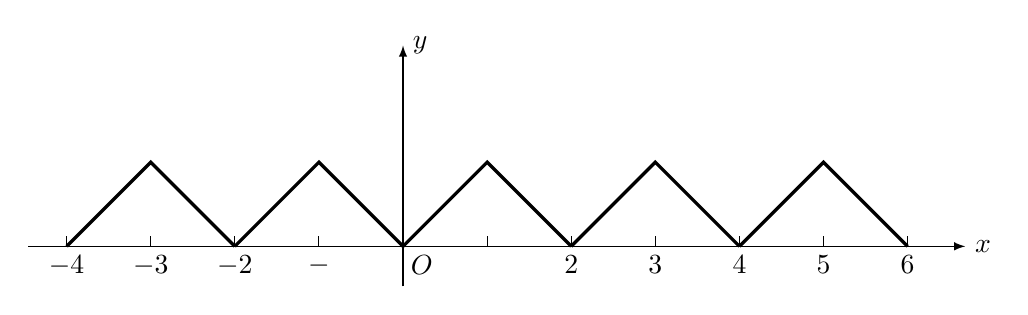
\begin{tikzpicture}[>=latex, scale=.34]
    \draw[->] (-14,0)--(21,0)node[right]{$x$};
    \draw[->] (0,-1.5)--(0,7.5)node[right]{$y$};
\foreach \x in {-4,-2,...,4}
{
    \draw[very thick] (\x*pi,0)--(\x*pi+pi,pi)--(\x*pi+pi+pi,0);
}
\foreach \x in {-4,-3,-2,2,3,4,5,6}
{
    \draw (\x*pi,0)node[below]{$\x\uppi$}--(\x*pi,.4);
}
\foreach \x/\xtext in {-1/-\uppi,1/\uppi}
{
    \draw (\x*pi,0)node[below]{$\xtext $}--(\x*pi,.4);
}
\node at (.7,-.7){$O$};


\end{tikzpicture}    
    \caption{}
\end{figure}
\end{solution}


\begin{Exercise}
\begin{question}
    \item 用反余弦的形式表示下列各式的角($x\in[0,\uppi]$)。
\begin{tasks}(2)
    \task $\cos\uppi =1$
    \task $\cos\frac{5\uppi}{3}=-\frac{1}{2}$
    \task $\cos(-3)=-0.9900$
    \task $\cos\frac{7\uppi}{6}=-\frac{\sqrt{3}}{2}$
    \task $\cos x=-0.8065$
    \task $\cos x=-1$
\end{tasks}

\item 决定下面差的符号:
\begin{tasks}(2)
  \task $\arccos0.7-\arccos0.5$
  \task $\arccos\left(-\frac{3}{5}\right)-\arccos\left(-\frac{3}{4}\right)$
  \task $\arccos\left(\sin\frac{\uppi}{12}\right)-\arccos\left(\sin\frac{\uppi}{13}\right)$
\end{tasks}
\item 不作计算,确定下列各比的符号:
\begin{tasks}(2)
    \task $\frac{\arcsin0.85-\arcsin0.8}{\arccos0.85-\arccos0.8}$
    \task $\frac{\uppi -2\arcsin(0.9)}{\uppi -2\arccos(0.1)}$
    \task $\frac{\arcsin(0.4)+\frac{\uppi}{6}}{\arcsin(0.6)-\frac{\uppi}{3}}$
\end{tasks}

\item 在同一个坐标系中,作函数$y=\arccos x$
和函数$y=\arccos\frac{x}{2}$
的图象,试根据函数图象说明当$x$为何值时,函数
的差$\arccos\frac{x}{2}-\arccos x$
取最大值、最小值、等于零。
\item 计算下列各式的值:
    \begin{tasks}(2)
\task $\sin \left(\arccos \frac{1}{2}\right)$
\task $\sin \left(\arccos \frac{3}{5}\right)$
\task $\tan \left(\arccos \frac{5}{13}\right)$
\task $\arcsin (\cos 1)$
\task $\arccos (\cos 2 \uppi)$
\task $\arccos \left(-\cos \frac{36}{7} \uppi\right)$
\task $\sin \left(\frac{1}{2} \arccos \frac{1}{2}\right)$
\task $\sin \left[3 \arccos \left(-\frac{\sqrt{3}}{2}\right)\right]$
\task $\sin \left[2 \arccos \left(-\frac{2 \sqrt{2}}{3}\right)\right]$
\task $\cos \left(\arcsin \frac{3}{5}-\arccos \frac{5}{13}\right)$    
\task $\sin\left[2\left(\arcsin\frac{\sqrt{5}}{3}-\arccos\frac{\sqrt{5}}{3}\right)\right]$
    \item $\tan\left(\arcsin\frac{1}{2}+\arccos\frac{\sqrt{3}}{2}\right)$
    \end{tasks}

\item 证明下面的恒等式:
\begin{enumerate}
\item 若$0<x<1$, 则:
$\arcsin x=\arccos\sqrt{1-x^2}$
\item 若$0<x<1$, 则:
$\arccos x=\arcsin\sqrt{1-x^2}$
\item 若$-1\leqslant x\leqslant 0$, 则:
$\arcsin x=-\arccos\sqrt{1-x^2}$
\item 若$-1\leqslant x\leqslant 0$, 则:
$\arccos x=\uppi-\arcsin\sqrt{1-x^2}$
\end{enumerate}

\item 解下面的方程:
    \begin{enumerate}
\item $\arccos x=\frac{\uppi}{3}$
\item $\arccos 2x=0.5$
\item $\arcsin x=\arccos x,\; |x|\leqslant 1$
\item $\arcsin x+\arcsin (1-x)=\arccos x$
\item $\arcsin x-\arccos x=\arcsin (3x-2)$
    \end{enumerate}

\item 当$-\frac{1}{2}\leqslant x\leqslant 0$时,求$f(x)
=\arccos x+x^2$的最小值。
\end{question}
\end{Exercise}

\section{反正切函数}

由正切函数$y=\tan x$的图象(图9.8)可以看出,函数$\tan x$
在每个开区间$\left(-\frac{\uppi}{2}+2k\uppi, \frac{\uppi}{2}+2k\uppi\right)$内,由$-\infty$上升到$+\infty$。
所以在每个这样的开区间里能带来一个反函数。


\begin{figure}[htp]
    \centering
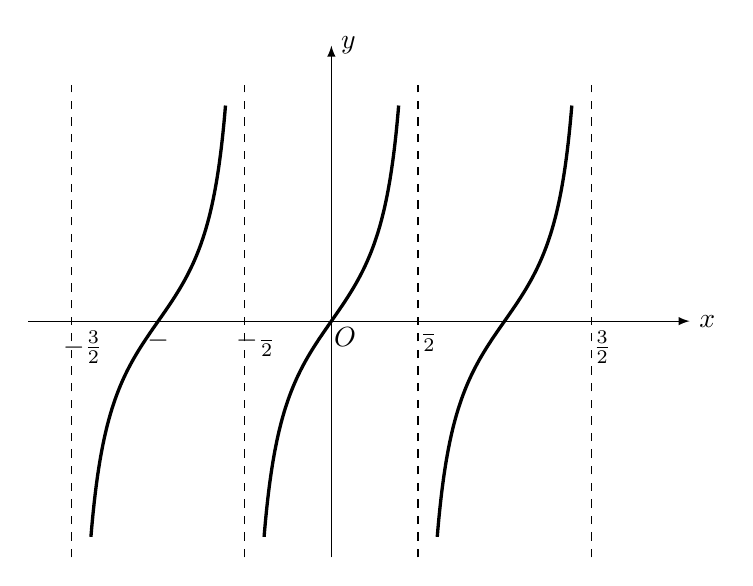
\begin{tikzpicture}[>=latex, xscale=.7]
    \draw[->] (-5.5,0)--(6.5,0)node[right]{$x$};
\draw[->] (0,-3)--(0,3.5)node[right]{$y$};
\foreach \x in {-.5,.5,1.5,-1.5}
{
    \draw[dashed] (\x*pi,-3)--(\x*pi,3);
}

\foreach \y in {-.5,.5,-1.5}
{
    \draw [domain=\y*pi+.35:(\y+1)*pi-.35, samples=1000, very thick] plot(\x, {tan(\x r)});
}

\node at (.25,-.2){$O$};
\node at (-pi,0)[below]{$-\uppi$};
\node at (pi,0)[above]{$\uppi$};

\node at (-.5*pi+.2,0)[below]{$-\frac{\uppi}{2}$};
\node at (.5*pi+.2,0)[below]{$\frac{\uppi}{2}$};
\node at (1.5*pi+.2,0)[below]{$\frac{3\uppi}{2}$};
\node at (-1.5*pi+.2,0)[below]{$-\frac{3\uppi}{2}$};
\end{tikzpicture}
    \caption{}

\end{figure}



\begin{blk}{定义3}
    函数$y=\tan x$在开区间$-\frac{\uppi}{2}<x<\frac{\uppi}{2}$
内的反函数叫做反正切函数 或 反正
切,记作
\[x=\arctan y\]
因为任何实数都可以作为正
切的值,所以反正切定义域是开区间$-\infty<y<+\infty$
\end{blk}

用几何名词来叙述反正
切的定义就是:在开区间
$(-\infty, +\infty)$内,数$y$的反
正切$x=\arctan y$是在开区间$-\frac{\uppi}{2}<x<\frac{\uppi}{2}$
内的一个角或弧,它的正切等于$y$,即:$\tan x=y$。

由定义和反函数定理直接得到反正切的性质如下:
\begin{enumerate}
    \item $\arctan (\tan x)=x, \qquad -\frac{\uppi}{2}<x<\frac{\uppi}{2}$
    
    $\tan (\arctan y)=y,\qquad -\infty<x<+\infty$
    \item $y=\arctan x,\; x\in\mathbb{R}$是单调递增的并且连续;
    \item $\arctan x$是奇函数,即
    \[\arctan (-x)=-\arctan x\]
    证明留给同学们去完成。
    \item 反正切函数$y=\arctan x,\; -\infty<x<+\infty$的图象如
    图5.9所示。
\end{enumerate}

\begin{figure}[htp]
    \centering
\begin{tikzpicture}[>=latex, scale=.7]
    \draw[->] (-5.5,0)--(6.5,0)node[right]{$x$};
    \draw[->] (0,-3)--(0,3)node[right]{$y$};
\draw[dashed] (-5.5,pi/2)--(6.5,pi/2);
\draw[dashed] (-5.5,-pi/2)--(6.5,-pi/2);

\draw [domain=-5.5:5.5, samples=100, very thick]plot(\x, {atan(\x)*pi/180});
\node at (.35,-.35){$O$};
\node at (0,2)[right]{$\frac{\uppi}{2}$};
\node at (0,-2)[right]{$-\frac{\uppi}{2}$};
\node at (5.5,pi/2-.3)[right]{$y=\arctan x$};
\end{tikzpicture}
    \caption{}
\end{figure}



\begin{example}
    求下列各式的值(口答):
\begin{tasks}(2)
    \task $\arctan 1$
    \task $\arctan (-1)$
    \task $\arctan \sqrt{3}$
    \task $\arctan (-\sqrt{3})$
\end{tasks}
\end{example}

\begin{solution}
\begin{enumerate}
    \item $\arctan 1=\frac{\uppi}{4}$,因为$\tan\frac{\uppi}{4}=1$,而且$-\frac{\uppi}{2}<\frac{\uppi}{4}<\frac{\uppi}{2}$
    \item $\arctan (-1)=-\frac{\uppi}{4}$,因为$\tan\left(-\frac{\uppi}{4}\right)=-1$,而且$-\frac{\uppi}{2}<-\frac{\uppi}{4}<\frac{\uppi}{2}$
    \item $\arctan \sqrt{3}=\frac{\uppi}{3}$,因为$\tan\frac{\uppi}{3}=\sqrt{3}$,而且$-\frac{\uppi}{2}<\frac{\uppi}{3}<\frac{\uppi}{2}$
    \item $\arctan (-\sqrt{3})=-\frac{\uppi}{3}$,因为$\tan\left(-\frac{\uppi}{3}\right)=-\sqrt{3}$,而且$-\frac{\uppi}{2}<-\frac{\uppi}{3}<\frac{\uppi}{2}$
\end{enumerate}
\end{solution}

\begin{example}
    求$\cos\left[\arctan\left(-\frac{3}{4}\right)\right]$
\end{example}

\begin{solution}
设$\alpha=\arctan\left(-\frac{3}{4}\right)$,其中$-\frac{\uppi}{2}<\alpha<\frac{\uppi}{2}$,则$\tan\alpha=-\frac{3}{4}$。

由于$-\frac{\uppi}{2}<\alpha<\frac{\uppi}{2}$和$\tan\alpha<0$,可以知道$\alpha$是第四象限的角。所以
\[\begin{split}
    \sec\alpha&=\sqrt{1+\tan^2\alpha}=\sqrt{1+\frac{9}{16}}=\frac{5}{4}\\
    \cos\alpha&=\frac{4}{5}
\end{split}\]
就是
\[\cos\left[\arctan\left(-\frac{3}{4}\right)\right]=\cos\alpha=\frac{4}{5}\]
\end{solution}

关于$y=\tan x$在其它单调区间内的反函数,请看下面命题。

\begin{blk}{命题}
    在开区间$\left(-\frac{\uppi}{2}+k\uppi ,\frac{\uppi}{2}+k\uppi 
\right)$,$k\in\mathbb{Z}$内$y=\tan x$
由$-\infty$上升到$+\infty$, 在这些区间上的反函数是
$x=\arctan y+k\uppi$。
\end{blk}

事实上,$x\in \left(-\frac{\uppi}{2}+k\uppi ,\frac{\uppi}{2}+k\uppi 
\right)$而
且
\[\tan x=\tan (\arctan y+k\uppi )=\tan (\arctan y)=y\]




\begin{example}
    求$\arctan 2+\arctan 3$的值。
\end{example}

\begin{solution}
    $\because\quad \frac{\uppi}{4}=\arctan 1<\arctan 2<\frac{\uppi}{2}$,$\frac{\uppi}{4}=\arctan 1<\arctan 3<\frac{\uppi}{2}$,

    $\therefore\quad \frac{\uppi}{2}<\arctan 2+\arctan 3<\uppi$。而且
\[\begin{split}
    \tan(\arctan 2+\arctan 3)&=\frac{\tan (\arctan 2)+\tan (\arctan  3)}{1-\tan(\arctan 2)\cdot \tan (\arctan 3)}\\
    &=\frac{2+3}{1-2\times 3}=-1
\end{split}\]
由于$\arctan (-1)\in \left(-\frac{\uppi}{2},0\right)$,于是
\[\arctan 2+\arctan 3=\arctan (-1)+\uppi=-\frac{\uppi}{4}+\uppi=\frac{3\uppi}{4}\]
\end{solution}

\begin{example}
    讨论 $y=\arctan (\tan x)$的图象。
\end{example}

\begin{solution}
函数$\arctan (\tan x)$的定义域是除去$x=\frac{\uppi}{2}+k\uppi,\; k\in\mathbb{Z}$
的实数集$\mathbb{R}$, 也就是无数个开区间$\left(-\frac{\uppi}{2}+k\uppi,\frac{\uppi}{2}+k\uppi\right),\; k\in\mathbb{Z}$
所组成的一个并集。因此函数$y=\arctan (\tan x)$的图象在
$x=\frac{\uppi}{2}+k\uppi,\; k\in\mathbb{Z}$这些点处间断。由于
\[\tan y=\tan[\arctan(\tan x)]\]
即:
$\tan y=\tan x$, 这里$-\frac{\uppi}{2}<y<\frac{\uppi}{2}$, $x\ne \frac{\uppi}{2}+k\uppi$。

所以,当$x\in\left(-\frac{\uppi}{2}+k\uppi,\frac{\uppi}{2}+k\uppi\right)$时,$x=y+k\uppi$, 也就是$y=x-k\uppi$。于是:
\begin{itemize}
    \item 当$x\in\left(-\frac{\uppi}{2},\frac{\uppi}{2}\right)$时,$y=x$;
    \item 当$x\in\left(\frac{\uppi}{2},\frac{3\uppi}{2}\right)$时,$y=x-\uppi$;
    \item 当$x\in\left(\frac{3\uppi}{2},\frac{5\uppi}{2}\right)$时,$y=x-2\uppi$;
    \item ………………
    \item 当$x\in\left(-\frac{3\uppi}{2},-\frac{\uppi}{2}\right)$时,$y=x+\uppi$;
    \item ………………
\end{itemize}
现在考虑间断点的情形:

当$\frac{\uppi}{2}+(k-)\uppi<x<\frac{\uppi}{2}+k\uppi$时,$y=x-k\uppi$, 于是当$x$
取每一个数列$\{x_n\}$从左边趋近$\frac{\uppi}{2}+k\uppi$ 时,记作
$x_n\to \left(\frac{\uppi}{2}+k\uppi \right)^-$, 
便有
\[\lim_{x_n\to \left(\tfrac{\uppi}{2}+k\uppi \right)^-}y=\lim_{x_n\to \left(\tfrac{\uppi}{2}+k\uppi \right)^-}(x_n-k\uppi)=\frac{\uppi}{2}+k\uppi-k\uppi=\frac{\uppi}{2}\]

当 $\dfrac{\uppi}{2}+k\uppi <x<\dfrac{\uppi}{2}+(k+1)\uppi$ 时,$y=x-(k+1)\uppi$。于
是当 $x$ 取每一个数列 $\{x_n\}$从右边趋近 $\dfrac{\uppi}{2}+k\uppi$ 时,记作 $x_n\to \left(\frac{\uppi}{2}+k\uppi\right)^+$,便有
\[\lim_{x_n\to \left(\tfrac{\uppi}{2}+k\uppi \right)^+}y=\lim_{x_n\to \left(\tfrac{\uppi}{2}+k\uppi \right)^+}[x_n-(k+1)\uppi]=\frac{\uppi}{2}+k\uppi-k\uppi-\uppi=-\frac{\uppi}{2}\]
因之,函数 $\arctan(\tan x)$ 在间断点$x=\dfrac{\uppi}{2}+k\uppi$ 处的左、右极限存在,其左极限等于 $\dfrac{\uppi}{2}$ 右极限等于 $-\dfrac{\uppi}{2}$,函数图象在这些间断点处,有一个等于 $\uppi$ 的跃度,它的图象如图9.10。

\begin{figure}
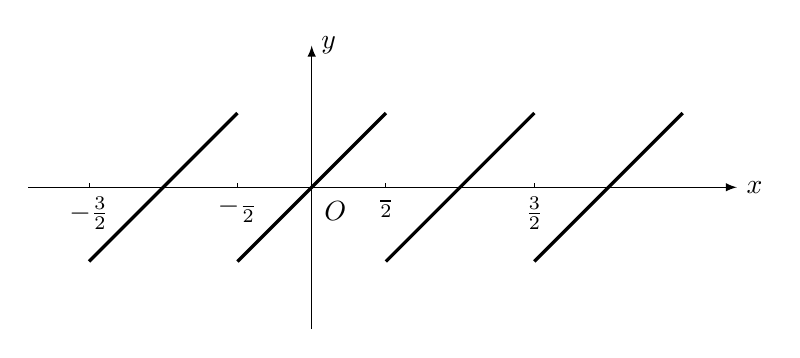
\begin{tikzpicture}[>=latex,scale=.6]
\draw[->] (-6,0)--(9,0)node[right]{$x$};
\draw[->] (0,-3)--(0,3)node[right]{$y$};    
\foreach \x/\xtext in {-1.5*pi/-\frac{3\uppi}{2},-.5*pi/-\frac{\uppi}{2},.5*pi/\frac{\uppi}{2},1.5*pi/\frac{3\uppi}{2}}
{
    \draw (\x,0)node[below]{$\xtext$}--(\x,.1);
}
\foreach \x in {-1.5*pi,-.5*pi,.5*pi,1.5*pi}
{
    \draw[very thick] (\x,-0.5*pi)--(\x+pi,0.5*pi);
}
\node at (.5,-.5){$O$};
\end{tikzpicture}
    \caption{}
\end{figure}
\end{solution}

\section{反余切函数}
由余切函数 $y=\cot x$ 的图象可以看出函数 $\cot x$ 在每个开区
间 $(k\uppi ,(k+1)\uppi ),\; k\in\mathbb{Z}$ 内,由 $+\infty$ 递减到 $-\infty$,所以在每个这样的开区间里,反函数是存在的。

\begin{Definition}
  函数 $y=\cot x$ 在开区间 $(0,\uppi )$ 内的反函数叫\emph{反余切函数或反余切},记作
\[x=\arccot y\]
它的定义域是开区间 $-\infty<y<+\infty$。
\end{Definition}

用几何名词来叙述反余切的定义便是:在开区间 $-\infty<y<+\infty$ 内,数 $y$ 的反余切 $x=\arccot y$ 是开区间 $0<x<\uppi$ 内的一个角或弧,它的余切等于 $y$,即 $\cot x=y$。

由反余切的定义和反函数定理得到反余切的性质如下:
\begin{enumerate}
  \item $\arccot (\cot x)=x,\; 0<x<\uppi ,\qquad \cot (\arccot y)=y,\; -\infty<y<+\infty$
  \item 反余切是递减的函数并且连续;
  \item $\arccot (-x)=\uppi -\arccot x$。

  这是因为$\arccot x$ 和 $\arccot (-x)$ 都属于 $(0,\uppi )$ 内的角,且
  \[0=\uppi -\uppi <\uppi - \arccot x<0+\uppi =\uppi \]
  又 $\cot (\uppi -\arccot x)=-\cot (\arccot x)=-x$,
  所以
  \[\uppi -\arccot x=\arccot (-x)\]
  即
  \[\arccot (-x)=\uppi -\arccot x\]
  \item 反余切 $y=\arccot x,\; -\infty<x<+\infty$ 的图象如\cref{fig:graph_arccot} 所示。
\end{enumerate}

\begin{figure}[htp]
    \centering
\begin{tikzpicture}[>=latex, scale=.8]
\draw[->] (-5,0)--(6,0)node[right]{$x$};
\draw[->] (0,-1)--(0,5)node[right]{$y$};
\draw (-5,pi)--(5,pi);
\node at (.25,-.25){$O$};
\node at (.2,pi)[above]{$\uppi$};
\node at (.2,0.5*pi)[above]{$\frac{\uppi}{2}$};
\draw [domain=.01:5, samples=100, very thick]plot(\x,{atan(1/\x)*pi/180});
\draw [domain=-5:-.01, samples=100, very thick]plot(\x,{atan(1/\x)*pi/180+pi});
\node at (-3.5,2.5){$y=\arccot x$};
\end{tikzpicture}    
    \caption{}\label{fig:graph_arccot}
\end{figure}



\begin{example}
  求下列各式的值:(口答)
  \begin{tasks}(2)
    \task $\arccot 1$
    \task $\arccot (- 1)$
    \task $\arccot \sqrt{3}$
    \task $\arccot \left(-\sqrt{3}\right)$
  \end{tasks}
\end{example}

\begin{solution}
\begin{tasks}
  \task $\arccot 1=\dfrac{\uppi}{4}$,因为 $\cot\dfrac{\uppi}{4}=1$,而且 $0<\dfrac{\uppi}{4}<\uppi$。
  \task $\arccot (- 1)=\uppi-\arccot 1=\uppi-\dfrac{\uppi}{4}=\dfrac{3\uppi}{4}$
  \task $\arccot \sqrt{3}=\dfrac{\uppi}{6}$,因为 $\cot\dfrac{\uppi}{6}=\sqrt{3}$,而且 $0<\dfrac{\uppi}{6}<\uppi$。
  \task $\arccot \left(-\sqrt{3}\right)=\uppi-\arccot\sqrt{3}=\uppi-\dfrac{\uppi}{6}=\dfrac{5\uppi}{6}$
\end{tasks}
\end{solution}

\begin{example}
  求 $\sin\left[\arccot\left(-\dfrac{1}{3}\right)\right]$ 的值
\end{example}

\begin{solution}
  设 $\arccot\left(-\dfrac{1}{3}\right)=\alpha$,其中 $0<\alpha<\uppi$,那么 $\cot\alpha=-\dfrac{1}{3}$。

  由于 $0<\alpha<\uppi$,$\cot\alpha<0$,可以知道 $\dfrac{\uppi}{2}<\alpha<\uppi$
\[\begin{split}
    \csc\alpha&=\sqrt{1+\cot^2\alpha}=\sqrt{1+\frac{1}{9}}=\sqrt{\frac{10}{9}}=\frac{\sqrt{10}}{3}\\
    \sin\alpha&=\frac{1}{\csc\alpha}=\frac{3}{\sqrt{10}}
\end{split}\]
$\therefore\quad \sin\left[\arccot\left(-\dfrac{1}{3}\right)\right]=\sin\alpha=\dfrac{3}{\sqrt{10}}=\dfrac{3\sqrt{10}}{10}$
\end{solution}

\begin{example}
    求证:对于任何实数 $x$ 有
\[\arctan x+\arccot x=\frac{\uppi}{2}\]
\end{example}

\begin{solution}
设 $\arctan x=\alpha$,其中 $-\dfrac{\uppi}{2}<\alpha<\dfrac{\uppi}{2}$,则 $\tan\alpha=x$。

又 $\cot\left(\dfrac{\uppi}{2}-\alpha\right)=\tan\alpha=x$,而 $0<\dfrac{\uppi}{2}-\alpha<\uppi$,所以 $\dfrac{\uppi}{2}-\alpha=\arccot x$。

将 $\alpha=\arctan x$ 代入上式,得到
\[\frac{\uppi}{2}-\arctan x=\arccot x\]
所以:$\arctan x+\arccot x=\dfrac{\uppi}{2},\quad x\in\mathbb{R}$
\end{solution}


\begin{example}
  证明 $\arctan 3+\arccot\left(-\dfrac{1}{5}\right)=\uppi-\arctan\dfrac{1}{8}$
\end{example}

\begin{solution}
设 $\alpha=\arctan 3$,其中 $0<\alpha<\dfrac{\uppi}{2}$,则 $\tan\alpha=3$。

又设 $\beta=\arccot\left(-\dfrac{1}{5}\right)$,其中 $\dfrac{\uppi}{2}<\beta<\uppi$,则:
\[\cot\beta=-\dfrac{1}{5},\qquad \tan\beta=-5\]
\[\begin{split}
 \tan\left[\arctan 3+\arccot\left(-\frac{1}{5}\right)\right]
&=\tan(\alpha+\beta)\\
&=\frac{\tan\alpha+\tan\beta}{1-\tan\alpha\cdot \tan\beta}\\
&=\frac{3+(-5)}{1-3(-5)}=-\frac{1}{8}
\end{split}\]
而且 $\dfrac{\uppi}{2}<\alpha+\beta<\dfrac{3\uppi}{2}$,
\[\therefore\quad \arctan 3+\arccot\left(-\frac{1}{5}\right)=\arctan\left(-\frac{1}{8}\right)+\uppi=\uppi-\arctan\frac{1}{8}\]
\end{solution}

\begin{Exercise}
\begin{question}
  \item 用反三角函数表示下面等式中的角。
  \begin{tasks}(2)
    \task $\displaystyle \tan\left(-\frac{\uppi}{4}\right)=-1$
    \task $\displaystyle \tan\left(\frac{7\uppi}{4}\right)=-1$
    \task $\displaystyle \tan\left(\frac{5\uppi}{6}\right)=-\frac{1}{\sqrt{3}}$
    \task $\displaystyle \tan\left(-\frac{3\uppi}{4}\right)=1$
    \task $\displaystyle \cot\frac{\uppi}{6}=\sqrt{3}$
    \task $\displaystyle \cot\left(-\frac{5\uppi}{4}\right)=-1$
    \task $\displaystyle \cot\left(-1\right)=-0.6421$
  \end{tasks}
  \item 指出下列各函数哪些是偶函数?哪些是奇函数?哪些既不是奇函数也不是偶函数。
  \begin{tasks}(2)
    \task $y=\arcsin x+2 \arctan x$
    \task $y=\arccos x+\arctan x$
    \task $y=\dfrac{\arcsin x}{\arccos x}$
    \task $y=\dfrac{\arctan x}{x}-x \arcsin x$
  \end{tasks}
  \item 计算下列各式的值:
  \begin{tasks}(2)
    \task  $\displaystyle \cos [\arctan(-\sqrt{3})]$;
    \task  $\displaystyle \sin (\arctan 2)$;
    \task  $\displaystyle \arctan(\tan2)$
    \task  $\displaystyle \arctan(\tan0.7 \uppi)$
    \task  $\displaystyle \tan\left(\arctan \frac{1}{4}-\arccot  5\right)$
    \task  $\displaystyle \sin \left(\arctan \frac{8}{15}-\arcsin \frac{7}{18}\right)$
    \task  $\displaystyle \tan\left[2 \arctan\left(-\frac{1}{2}\right)\right]$
    \task  $\displaystyle \cos \left[2 \arctan \frac{1}{4}+\arccos \frac{3}{5}\right]$
  \end{tasks}
  \item 检验下列各等式是否正确。
  \begin{tasks}(2)
    \task $\displaystyle \arcsin \frac{15}{17}=\arccos \frac{8}{17}$
    \task $\displaystyle \arcsin \frac{4}{5}=\arccot\frac{3}{4}$
    \task $\displaystyle \arcsin \left(-\frac{7}{25}\right)=-\arctan \frac{7}{24}$
    \task $\displaystyle \arccos \left(-\frac{9}{41}\right)=\uppi-\arcsin \frac{40}{41}$
    \task $\displaystyle \arctan \frac{2}{3}+\arctan \frac{1}{5}=\frac{\uppi}{4}$
    \task $\displaystyle \arccot\frac{1}{9}+\arccot\frac{4}{5}=\frac{3}{4} \uppi$
    \task! $\displaystyle 2 \arctan \frac{1}{3}+\arctan \frac{1}{4}=\arctan \frac{16}{13}$
    \task! $\displaystyle \arcsin \frac{7}{25}+\frac{1}{2} \arccos \frac{7}{25}=\arccos \frac{3}{5}$
  \end{tasks}   
  \item 证明下面恒等式:
  \begin{question}[label=\alph*),listparindent=0pt]
    \item 若 $0<x<1$, 那么
    \[\arcsin x=\arccos\sqrt{1-x^2}=\arctan\frac{x}{\sqrt{1-x^2}}=\arccot\frac{\sqrt{1-x^2}}{x}\]
    \item 若 $0<x<1$, 那么
    \[\arccos x=\arcsin\sqrt{1-x^2}=\arctan\frac{\sqrt{1-x^2}}{x}=\arccot\frac{x}{\sqrt{1-x^2}}\]
    \item 若 $x>0$, 那么
    \[\arctan x=\arccot \frac{1}{x}=\arcsin\frac{x}{\sqrt{1+x^2}}=\arccos\frac{1}{\sqrt{1+x^2}}\]
    \item 若 $x>0$, 那么
    \[\arccot x=\arctan \frac{1}{x}=\arcsin\frac{1}{\sqrt{1+x^2}}=\arccos\frac{x}{\sqrt{1+x^2}}\]
    \item 若 $|x|\leqslant 1$,那么 $\arcsin x=\arctan\dfrac{x}{\sqrt{1-x^2}}$

    若 $-1\leqslant x\leqslant 0$,那么 $\arcsin x=-\arccos{\sqrt{1-x^2}}$

    若 $-1\leqslant x< 0$,那么 $\arcsin x=\arctan\dfrac{\sqrt{1-x^2}}{x}-\uppi$

    \item 若 $-1\leqslant x\leqslant 0$,那么 $\arccos x=\uppi-\arcsin{\sqrt{1-x^2}}$

    若 $-1\leqslant x< 0$,那么 $\arccos x=\uppi+\arctan\dfrac{\sqrt{1-x^2}}{x}$

    若 $|x|\leqslant 1$,那么 $\arccos x=\arctan\dfrac{x}{\sqrt{1-x^2}}$

    \item 若 $x<0$, 那么 $\arctan x=\arccot \dfrac{1}{x}-\uppi$

    若 $x<0$, 那么 $\arccot x=\uppi+\arctan\dfrac{1}{x}$

    \item 若 $x\geqslant 0$,$\dfrac{1}{2}\arccos(2x^2-1)=\arccos x$
    \item 若 $x\geqslant 1$,$2\arctan x+\arcsin\dfrac{2x}{1+x^2}=\uppi$
  \end{question}
  \item 作函数$y=x-\arctan(\tan x)$的草图。
  \item 解下列方程:
  \begin{tasks}(2)
    \task $\displaystyle \arctan x=\frac{\uppi}{4}$
    \task $\displaystyle \arctan x=\frac{\uppi}{2}$
    \task $\displaystyle \arctan x=-\frac{\uppi}{2}$
    \task $\displaystyle \arctan x^2=3$
    \task $\displaystyle \arctan 2x+\arctan 3x=\frac{3\uppi}{4}$
    \task! $\sin\Big\{2\arccos\big[\cot(2\arctan x)\big]\Big\}=0$
  \end{tasks}
  \item 若 $\arctan x+\arctan y+ \arctan z=\uppi$,求证:$x+y+z=xyz$。
  \item 求证:
  \[\arctan x+\arctan\frac{1-x}{1+x}=\begin{cases}
    \dfrac{\uppi}{4},& x>-1\\
    -\dfrac{3\uppi}{4},& x<-1
  \end{cases}\]
\end{question}
\end{Exercise}

\section{最简单的三角方程}
下列方程 $\sin x=a$,$\cos x=a$,$\tan x=a$,$\cot x=a$ 中的 $a$ 为已给的实数,$x$ 是未知数,是最简单的三角方程。适合其中某
个方程的 $x$ 值叫做这个方程的解或根。例如,诸角:$x=\ang{30}$;$x=\ang{150}$;$x=\ang{390}$;$x=\ang{510}$ 等等,为三角方程
$\sin x=\dfrac{1}{2}$ 的解,因为,
\[\sin\ang{30}=\sin\ang{30}=\sin\ang{30}=\sin\ang{30}=\frac{1}{2}\]

解三角方程就是求它的一切解,根据前一节内容知道,已知三角函数值 $a$ 所对应的角的值,如果存在的话,有无穷多个,所以每一个三角方程都有无穷多个解,它的所有解简称为通解。

在本节中,我们来解上面所示的最简单三角方程,从以后的例子即将明白,解三角方程归根到底化为解最简单的三角方程。

\subsection{最简单三角方程的解}
\subsubsection{$\sin x=a$ 的解}
分 $|a|\leqslant 1$ 和 $|a|>1$ 的情形来考虑:

\textbf{第一种情形:} $0<a<1$
 
在坐标系 $x$-$O$-$y$ 中,以原点 $O$ 为圆心作一单位圆,在 $Oy$ 轴上作出纵坐标等于 $a$ 的 $Q$ 点,并过 $Q$ 点引平行于 $Ox$ 轴的直线,交单位圆周于 $A$和$B$二点,如图9.12, $P_0$为$(1,0)$,
$\angle P_0OA=\arcsin a$和$\angle P_0OB=\uppi-\arcsin a$的正弦都等于$a$,
所以$\arcsin a$ 和$\uppi-\arcsin a$是方程$\sin x=a$的特解,为求方程
$\sin x=a$的通解,可将$2k\uppi$加于此两角中的每一个而得到,其
中$k\in\mathbb{Z}$。 因此,原方程的通解是
\[\begin{split}
   x_1&=2k\uppi +\arcsin a\\
x_2&=2k\uppi +\uppi -\arcsin a=(2k+1)\uppi -\arcsin a 
\end{split}\]
合并起来,可写成
\[x=k\uppi +(-1)^k\arcsin a,\qquad k\in\mathbb{Z}\]

我们约定,在三角方程的通解中,“$k\in\mathbb{Z}$”以后不再
交代。

\begin{figure}[htp]\centering
    \begin{minipage}[t]{0.48\textwidth}
    \centering
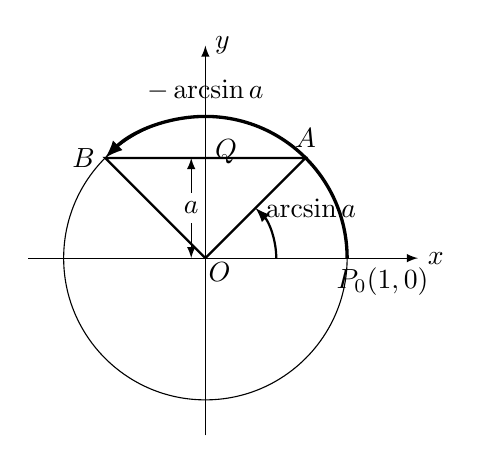
\begin{tikzpicture}[>=latex, scale=.9]
\draw [<->](-.2,0)--node[fill=white]{$a$}(-.2,1.414);
\draw[->] (-2.5,0)--(3,0)node[right]{$x$};
\draw[->] (0,-2.5)--(0,3)node[right]{$y$};
\draw (0,0) circle (2);
\draw[thick] (0,0)--(45:2)node[above]{$A$}--(135:2)node[left]{$B$}--(0,0);
\node at (.2,-.2){$O$};
\node at (0,1.5)[right]{$Q$};
\node at (2.5,0)[below]{$P_0(1,0)$};
\draw[->,  thick] (1,0) arc (0:45:1)node[right]{$\arcsin a$};
\draw[->, very thick] (2,0) arc (0:135:2);
\node at (0,2)[above=2pt]{$\uppi-\arcsin a$};
    \end{tikzpicture}
    \caption{}
    \end{minipage}
    \begin{minipage}[t]{0.48\textwidth}
    \centering
    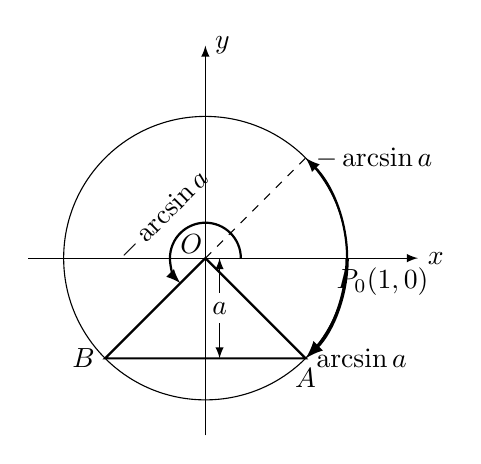
\begin{tikzpicture}[>=latex, scale=.9]
\draw [<->](.2,0)--node[fill=white]{$a$}(.2,-1.414);
\draw[->] (-2.5,0)--(3,0)node[right]{$x$};
\draw[->] (0,-2.5)--(0,3)node[right]{$y$};
\draw (0,0) circle (2);
\node at (-.2,.2){$O$};
\node at (2.5,0)[below]{$P_0(1,0)$};
\draw[thick] (0,0)--(-45:2)node[below]{$A$}--(-135:2)node[left]{$B$}--(0,0);
\draw[dashed] (0,0)--(45:2);
\draw[->, thick] (2,0) arc (0:45:2)node[right]{$-\arcsin a$};
\draw[->, very thick] (2,0) arc (0:-45:2)node[right]{$\arcsin a$};
\draw[->, thick] (.5,0) arc (0:180+45:.5);
\node at (-.6,.6)[rotate=45]{$\uppi-\arcsin a$};

    \end{tikzpicture}
    \caption{}
    \end{minipage}
    \end{figure}


\emph{第二种情形:} $-1<a<0$

用同样的方法作图,如图9.13所示:
$\angle P_0OA=\arcsin a$和$\angle P_0OB=\uppi-\arcsin a$是方程$\sin x=a,\; -1<a<0$的特解,因此,原方程的通解仍是
\[\begin{split}
  x_1&=2k\uppi +\arcsin a\\
x_2&=2k\uppi +\uppi -\arcsin a=(2k+1)\uppi -\arcsin a  
\end{split}\]
合并起来,可写成
\[x=k\uppi +(-1)^k\arcsin a\]

\emph{第三种情形:} $a=1$

方程$\sin x=1$的特解是$x=\frac{\uppi}{2}$,
因此,原方程的通解是
\[x=\frac{\uppi}{2}+2k\uppi\quad \text{或者}\quad x=90^{\circ}+k\cdot 360^{\circ}\]

\emph{第四种情形:} $a=-1$

\[\sin x=-1\]
特解:$x=-\frac{\uppi}{2}$(或$x=-90^{\circ}$),

通解:$x=-\frac{\uppi}{2}+2k\uppi$ (或$x=-90^{\circ}+k\cdot 360^{\circ}$)。

\emph{第五种情形:} $a=0$

\[\sin x=0\]
特解:$x_1=0$和$x_2=\uppi$。

通解:$x_1=2k\uppi$和$x_2=\uppi +2k\uppi =(2k+1)\uppi$,
合并成:\[x=k\uppi\]

\emph{第六种情形:} $|a|>1$

在这种情形下,$\sin x=a$没有解。

将结果总结于下表内
\begin{center}
\begin{tabular}{c|c}
    \hline
$a$的数值& 方程$\sin x=a$的解\\
    \hline
$-1<a<0,\; 0<a<1$ & $x=k\uppi +(-1)^k\arcsin a$\\
$a=-1$& $x=-\frac{\uppi}{2}+2k\uppi$\\
$a=0$&   $x=k\uppi$\\
$a=1$& $x=\frac{\uppi}{2}+2k\uppi$\\
$|a|>1$ & 方程无解\\
    \hline
\end{tabular}   
\end{center}

\begin{example}
    解方程$\sin x=\frac{1}{2} $
\end{example}

\begin{solution}
    \[x=k\uppi+(-1)^k\arcsin\frac{1}{2}=k\uppi+(-1)^k\frac{\uppi}{6}\]
    或者\[x=k\cdot 360^{\circ}+(-1)^k\cdot 30^{\circ},\qquad (k\in\mathbb{Z})\]
\end{solution}


\begin{example}
    解方程$\sin x=-\frac{1}{2} $
\end{example}

\begin{solution}
\[x=k\uppi+(-1)^k\arcsin\left(-\frac{1}{2}\right)=k\uppi+(-1)^{k+1}\frac{\uppi}{6}\]
    或者\[x=k\cdot 360^{\circ}+(-1)^{k+1}\cdot  30^{\circ},\qquad (k\in\mathbb{Z})\]
\end{solution}


\begin{example}
    解方程$\sin (2x-1)=\frac{\sqrt{3}}{2} $
\end{example}

\begin{solution}
\[\begin{split}
   2x-1&=k\uppi+(-1)^k \arcsin\frac{\sqrt{3}}{2}\\ 
2x&=k\uppi+(-1)^k \cdot \frac{\uppi}{3}+1\\
  x &=k\cdot\frac{\uppi}{2}+(-1)^k\cdot \frac{\uppi}{6}+\frac{1}{2} ,\qquad (k\in\mathbb{Z})
 \end{split}\]   
\end{solution}

\subsubsection{$\cos x=a$的解}

\emph{第一种情形:} $0<a<1$
在$Ox$轴上作出横坐标等于$a$的$P$点,并过$P$点作平行于$Oy$
轴的直线交单位圆周于$C$和$D$二点,$P_0$为$(1,0)$(图9.14)。
$\angle P_0OC=\arccos a$和$\angle P_0OD=-\arccos a$的余弦等于$a$, 故它
们是方程的解,原方程的通解是
\[x=2k\uppi\pm \arccos a\]

\emph{第二种情形:} $-1<a<0$
作类似的图形,如图9.15同样可得原方程的通解是
\[x=2k\uppi\pm \arccos a\]

\begin{figure}[htp]\centering
    \begin{minipage}[t]{0.48\textwidth}
    \centering
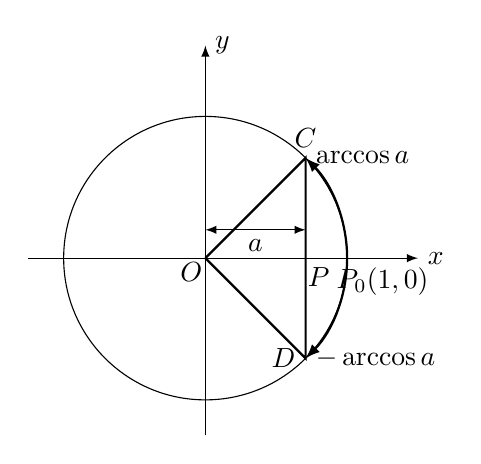
\begin{tikzpicture}[>=latex, scale=.9]
\draw [<->](0,.4)--node[below]{$a$}(1.414,.4);
\draw[->] (-2.5,0)--(3,0)node[right]{$x$};
\draw[->] (0,-2.5)--(0,3)node[right]{$y$};
\draw (0,0) circle (2);
\draw[thick] (0,0)--(45:2)node[above]{$C$}--(-45:2)node[left]{$D$}--(0,0);
\node at (-.2,-.2){$O$};
\node at (1.6,0)[below]{$P$};
\node at (2.5,0)[below]{$P_0(1,0)$};
\draw[->,  thick] (2,0) arc (0:45:2)node[right]{$\arccos a$};
\draw[->,  thick] (2,0) arc (0:-45:2)node[right]{$-\arccos a$};
    \end{tikzpicture}
    \caption{}
    \end{minipage}
    \begin{minipage}[t]{0.48\textwidth}
    \centering
    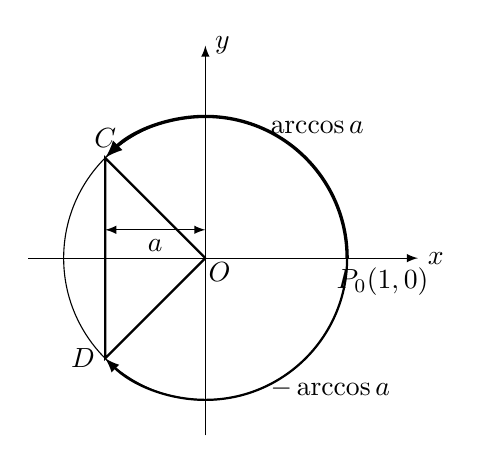
\begin{tikzpicture}[>=latex, scale=.9]
\draw [<->](0,.4)--node[below]{$a$}(-1.414,.4);
\draw[->] (-2.5,0)--(3,0)node[right]{$x$};
\draw[->] (0,-2.5)--(0,3)node[right]{$y$};
\draw (0,0) circle (2);
\draw[thick] (0,0)--(135:2)node[above]{$C$}--(-135:2)node[left]{$D$}--(0,0);
\node at (.2,-.2){$O$};
\node at (2.5,0)[below]{$P_0(1,0)$};
\draw[->, very thick] (2,0) arc (0:135:2);
\draw[->,  thick] (2,0) arc (0:-135:2);
\node at (67:2)[right]{$\arccos a$};
\node at (-67:2)[right]{$-\arccos a$};
    \end{tikzpicture}
    \caption{}
    \end{minipage}
    \end{figure}

\emph{第三种情形:} $a=1$

\[\cos x=1\]

方程的特解:$x=0$, 方程的通解:$x=2k\uppi$。

\emph{第四种情形:} $a=-1$

\[\cos x=-1\]
方程的特解:$x=\uppi$, 方程的通解:$x=\uppi+2k\uppi=(2k+1)\uppi$。

\emph{第五种情形:} $a=0$
\[\cos x=0\]
方程的特解:$x_1=\frac{\uppi}{2}$和$x_2=-\frac{\uppi}{2}=\frac{\uppi}{2}-\uppi$。

方程的通解:$x=\frac{\uppi}{2}+k\uppi$。

\emph{第六种情形:} $|a|>1$

在这种情形下,方程$\cos x=a$无解。

将结果综合于下表内:
\begin{center}
    \begin{tabular}{c|c}
        \hline
    $a$的数值& 方程$\cos x=a$的解\\
        \hline
    $-1<a<0,\; 0<a<1$ & $x=2k\uppi \pm \arccos a$\\
    $a=-1$& $x=(2k+1)\uppi$\\
    $a=0$&   $x=\frac{\uppi}{2}+k\uppi$\\
    $a=1$& $x=2k\uppi$\\
    $|a|>1$ & 方程无解\\
        \hline
    \end{tabular}   
    \end{center}



\begin{example}
    解方程$2\cos x+1=0$
\end{example}

\begin{solution}
    化简为$\cos x=-\frac{1}{2}$,通解如下:
\[\begin{split}
    x&=2k\uppi\pm\arccos\left(-\frac{1}{2}\right)\\
    &=2k\uppi\pm \left(\uppi-\arccos\frac{1}{2}\right)\\
    &=2k\uppi\pm \left(\uppi-\frac{\uppi}{3}\right)\\
    &=2k\uppi\pm \frac{2\uppi}{3}
\end{split}\]
\end{solution}


\begin{example}
    解方程$\cos\left(\frac{x}{4}+\frac{\uppi}{5}\right)=0$
\end{example}

\begin{solution}
    \[\begin{split}
        \frac{x}{4}+\frac{\uppi}{5}&=\frac{\uppi}{2}+k\uppi\\
        \frac{x}{4}&=\frac{\uppi}{2}-\frac{\uppi}{5}+k\uppi=\frac{3\uppi}{10}+k\uppi\\
        x&=4\left(\frac{3\uppi}{10}+k\uppi\right)=\frac{6\uppi}{5}+4k\uppi
    \end{split}
    \]
\end{solution}

\subsubsection{$\tan x=a$的解}

如图9.16所示,$\angle P_0OA=\arctan a$和$\angle P_0OB=\uppi+\arctan a$
是方程的解,因为它们的正切等于 $a$。原方程的通解是
\[x=k\uppi+\arctan a\]


\begin{example}
    解方程$\tan x=-1$    
\end{example}

\begin{solution}
\[x=k\uppi+\arctan(-1)=k\uppi-\arctan1=k\uppi-\frac{\uppi}{4}\]
\end{solution}

\subsubsection{$\cot x=a$的解}

如图9.17所示,$\angle P_0OA=\arccot a$ 和 $\angle P_0OB=\uppi+\arccot a$ 是方
程的特解,因为它们的余切等于$a$。原方程的通解是
\[x=k\uppi+\arccot a,\qquad (k\in\mathbb{Z})\]

\begin{figure}[htp]\centering
    \begin{minipage}[t]{0.48\textwidth}
    \centering
\begin{tikzpicture}[>=latex, scale=.9]
\draw [|<->|](2.2,0)--node[right]{$a$}(2.2,2);
\draw[->] (-2.5,0)--(3,0)node[right]{$x$};
\draw[->] (0,-2.5)--(0,3)node[right]{$y$};
\draw (0,0) circle (2);
\draw[thick] (-135:2)node[below]{$B$}--(0,0)--(45:2)node[above]{$A$}--(2,2);
\node at (.2,-.2){$O$};
\node at (2.7,0)[below]{$P_0(1,0)$};
\draw[->, very thick] (2,0) arc (0:45:2);
\draw[->,  thick] (2,0) arc (0:180+45:2);
\node at (1,.3){$\arctan a$};
\node at (-2,1.5){$\uppi+\arctan a$};
\draw(2,-2.5)--(2,3)node[right]{正切线};
    \end{tikzpicture}
    \caption{}
    \end{minipage}
    \begin{minipage}[t]{0.48\textwidth}
    \centering
    \begin{tikzpicture}[>=latex, scale=.9]
\draw [|<->|](0,2.2)--node[above]{$a$}(2,2.2);
\draw[->] (-2.5,0)--(3,0)node[right]{$x$};
\draw[->] (0,-2.5)--(0,3)node[right]{$y$};
\draw (0,0) circle (2);
\draw[thick] (-135:2)node[below]{$B$}--(0,0)--(45:2)node[above]{$A$}--(2,2);
\node at (.2,-.2){$O$};
\node at (2.7,0)[below]{$P_0(1,0)$};
\draw[->, very thick] (2,0) arc (0:45:2);
\draw[->,  thick] (2,0) arc (0:180+45:2);
\node at (23:2.2)[right]{$\arccot a$};
\node at (-2,1.5){$\uppi+\arccot a$};
\draw(-2.5,2)--(3,2)node[above]{余切线};
    \end{tikzpicture}
    \caption{}
    \end{minipage}
    \end{figure}


\begin{example}
    解方程 $9\cot^2 2x-25=0$
\end{example}

\begin{solution}
    \[\begin{split}
        \cot^2 2x&=\frac{25}{9}\\
        \cot 2x&=\pm\frac{5}{3}\approx \pm 1.6667
    \end{split}\]
由$\cot 2x=1.6667$,得:
\[\begin{split}
    2x&=30^{\circ}58'+k\cdot 180^{\circ}\\
    x&=15^{\circ}29'+k\cdot 90^{\circ}
\end{split}\]
由$\cot 2x=-1.6667$,得:
\[\begin{split}
    2x&=(180^{\circ}-30^{\circ}58')+k\cdot 180^{\circ}\\
    2x&=149^{\circ}2'+k\cdot 180^{\circ}\\
    x&=74^{\circ}31'+k\cdot 90^{\circ}
\end{split}\]
$\therefore\quad $原方程的近似解是:
\[x=15^{\circ}29'+k\cdot 90^{\circ}\quad \text{和}\quad x=74^{\circ}31'+k\cdot 90^{\circ}\]
\end{solution}

\subsection{解简单三角方程的例子}
在本节中,我们来研究某些三角方程的解法。解这些方程时,一般是应用三角函数的恒等变形和解代数方程的一般知识把它归结成解一个或几个最简单的三角方程,从而求出所有解。在解三角方程的过程中,应当避免作可能破坏方程同解性的变形,如果这类变形不可避免,则需研究哪些根会失掉,哪些根是增根,对最终方程的诸解,应当进行检验,确定它们是否是原方程的解。下面通过例子来阐明。

\subsubsection{含有同角的同名三角函数的方程}
\begin{example}
  解方程 $2\cos^2x+\cos x-1=0$
\end{example}

\begin{solution}
把方程看作关于未知数为 $\cos x$ 的二次方程,按照二次方程的解法,可得
\[\cos x=\frac{-1\pm\sqrt{1+8}}{4}=\frac{-1\pm 3}{4}\]
由此得:$\cos x=\dfrac{1}{2}$ 或 $\cos x=-1$。

由 $\cos x=\dfrac{1}{2}$,得:$x=2k\uppi+\frac{\uppi}{3}$;由 $\cos x=-1$,得:$x=(2k+1)\uppi$。

$\therefore\quad $ 原方程的解集是
\[\left\{x\big| x=2k\uppi\pm \frac{\uppi}{3}\right\}\cup \left\{x\big| x=(2k+1)\uppi \right\}\]
\end{solution}

\begin{example}
  解方程 $2\sin^2x+2\sin x-\sqrt{3}\sin x=\sqrt{3}$
\end{example}

\begin{solution}
\textbf{解法1:} 把一切项都移至左端,得:$2\sin^2x+\left(2-\sqrt{3}\right)\sin x-\sqrt{3}=0$。解关于 $\sin x$ 的二次方程,得
\[\begin{split}
\sin x&=\frac{-2+\sqrt{3}\pm \sqrt{\left(2-\sqrt{3}\right)^2+8\sqrt{3}}}{4}\\
&=\frac{-2+\sqrt{3}\pm \sqrt{4+4\sqrt{3}+3}}{4}\\
&=\frac{-2+\sqrt{3}\pm \sqrt{\left(2+\sqrt{3}\right)^2}}{4}\\
&=\frac{-2+\sqrt{3}\pm \left(2+\sqrt{3}\right)}{4}
\end{split}\]
由此得
\[\sin x=\frac{\sqrt{3}}{2}\quad \text{或}\quad \sin x=-1\]

由 $\sin x=\dfrac{\sqrt{3}}{2}$ 得:$x=k\cdot \ang{180}+(-1)^k\cdot \ang{60}$。

由 $\sin x=-1$ 得:$x=-\ang{90}+k\cdot \ang{360}$。

$\therefore\quad $ 原方程的解集是
\[\left\{x|x=k\cdot 180^{\circ}+(-1)^k\cdot 60^{\circ}\right\}\cup \left\{x|x=-90^{\circ}+k\cdot 360^{\circ}\right\}\]
这里 $k\in\mathbb{Z}$。

\emph{解法2:} 把一切项都移至左端得:$2\sin^2x+2\sin x-\sqrt{3}\sin x-\sqrt{3}=0$

方程左端可以分解因式:
\[\begin{split}
    2\sin x(\sin x+1)-\sqrt{3}(\sin x+1)&=0\\
    (\sin x+1)\left(2\sin x-\sqrt{3}\right)&=0
\end{split}\]

若两个因式的乘积等于零,则至少有一个因式等于零,同时应当满足下列条件:对于使第一个因式为零的解,应当使方程的第二个因式有确定的值。上面的方程可分为这样的
两个方程:
\[2\sin x-\sqrt{3}=0\quad \text{或}\quad \sin x+1=0\]
分别由$\sin x=\frac{\sqrt{3}}{2} $和$\sin x=-1$,得到:
\[x=k\uppi+(-1)^k \cdot\frac{\uppi}{3}\quad \text{和}\quad x=-\frac{\uppi}{2}+2k\uppi\]

把$x=k\uppi+(-1)^k \cdot\frac{\uppi}{3}$代入$\sin x+1$中,有确定值,同
样把$x=-\frac{\uppi}{2}+2k\uppi$代入$2\sin x-\sqrt{3}$中,也有确定值,所以
原方程的解集是
\[\left\{x\Big|x=k\uppi+(-1)^k \cdot\frac{\uppi}{3}\right\}\bigcup \left\{x\Big|x=-\frac{\uppi}{2}+2k\uppi\right\}\]
\end{solution}

一般的情况下,在三角方程中,不只有一个三角函数,
我们可以利用同一个角的各三角函数值之间的关系式,把方
程中未知角的各三角函数都用某一个三角函数表示出来,这
样,就把所解的三角方程先归结到多项式方程的问题。

\begin{example}
    解方程 $\sin^2 x+\cos x+1=0$
\end{example}

\begin{solution}
$\because\quad \sin^2 x=1-\cos^2x$,\qquad $\therefore\quad $原方程可化为:
\[\begin{split}
    \cos^2x-\cos x-2&=0\\
    \cos x&=\frac{1\pm 3}{2}
\end{split}\]
由此得到
\[\cos x=2\quad \text{或}\quad \cos x=-1\]

$\because\quad \cos x=2>1$,\qquad  $\therefore\quad $方程无解。

由$ \cos x=-1$,得:$x=(2k+1)\uppi$

$\therefore\quad $原方程的解集是$\{x|x=(2k+1)\uppi,\; k\in\mathbb{Z}\}$。
\end{solution}

\begin{example}
    解方程$\cos x-\sin x=0$
\end{example}

\begin{solution}
    如果用$\cos x$表示$\sin x$或用$\sin x$表示$\cos x$, 那么我们就
    得到根式方程,为了避免这点,可以用$\cos x$去除方程的两
    边,得到
    \[1-\tan x=0\]
    因为原方程的解不含有$\cos x=0$的解,所以我们有根据这样
    做。事实上,由$\cos x=0$, 得到
    $x=\frac{\uppi}{2}+k\uppi$, 代入$\cos x-\sin x$中,有
   \[ \cos\left(\frac{\uppi}{2}+k\uppi \right)-sin\left(\frac{\uppi}{2}+k\uppi \right)=0-(-1)^k\sin \frac{\uppi}{2}=(-1)^{k+1}\ne 0\]
    不满足原方程。
    
    因此,用$\cos x$去除原方程的两边,得到和原方程同解的方程
    \[\tan x=1\]
    由此,
   $ x=k\uppi +\frac{\uppi}{4}$。

   所以原方程的解集是
$\left\{x\Big|x=k\uppi+\frac{\uppi}{4},\; k\in\mathbb{Z}\right\}$
\end{solution}

\begin{rmk}
当解$\cos x-\sin x=0$时,也可以把
$\cos x$提出括号之外,而不用$\cos x$去除两端,原方程可写成下面的形式
$$\cos x (1-\tan x)=0$$
由此得到
$$\cos x=0\quad \text{或}\quad \tan x=1$$
但是使$\cos x=0$的解:$x=\frac{\uppi}{2}+k\uppi$却使因式$1-\tan x$无意义,这就表示$x=\frac{\uppi}{2}+k\uppi$是原方程的增根,因此必须舍去,同样我们得到原方程的同解方程
$\tan x=1$。

对于例9.29这种方程的解法还可以应用到下面更一般的类
型上去。

左端是关于$\sin x$和$\cos x$的齐次多项式右端是零的方程,
称为\emph{齐次方程},例9.29的方程是齐次方程的一个特例。
\end{rmk}




\begin{example}
    解齐次方程$2\sin^2x-7\sin x\cos x+6\cos^2x=0$
\end{example}

\begin{solution}
用$\cos^2x$除原方程的两端,得
\[2\tan^2 x-7\tan x+6=0\]
由此得$\tan x=2\quad \text{或}\quad \tan x=1.5$

由$\tan x=2$得
\[x\approx k\cdot 180^{\circ}+63^{\circ}26'\]

由$\tan x=1.5$得
\[x\approx k\cdot 180^{\circ}+56^{\circ}19'\]
$\therefore\quad $原方程的解集是:
\[\left\{x\big|x=k\cdot 180^{\circ}+63^{\circ}26' \right\}\cup \left\{x\big|x=k\cdot 180^{\circ}+56^{\circ}19' \right\}\]
或者
\[\left\{x\big|x=k\uppi+\arctan 2 \right\}\bigcup\left\{x\big|x=k\uppi+\arctan\frac{3}{2} \right\}\]

又这样的方程
$2\sin^2x+5\sin x\cos x+\cos^2x=4$
也可以归入齐次方程,因为原方程可写成
\[2\sin^2x+5\sin x\cos x+\cos^2x-4(\cos^2x+\sin^2x)=0\]
化简得
\[2\sin^2x-5\sin x\cos x+3\cos^2x=0\]
\end{solution}

\begin{example}
    解方程$8\sin^2\frac{x}{2}+3\sin x-4=0$
\end{example}

\begin{solution}
    原方程可以变形为齐次方程
\[8\sin^2\frac{x}{2}+6\sin \frac{x}{2}\cos\frac{x}{2}-4\left(\sin^2\frac{x}{2}+\cos^2\frac{x}{2}\right)=0\]
化简得:$2\sin^2\frac{x}{2}+3\sin\frac{x}{2}\cos\frac{x}{2}-2\cos^2\frac{x}{2}=0$。

两边除以$\cos^2\frac{x}{2}$, 得
    \[2\tan^2\frac{x}{2}+3\tan\frac{x}{2}-2=0\]
所以$\tan\frac{x}{2}=-2\quad \text{或}\quad \tan\frac{x}{2}=\frac{1}{2}$。

由$\tan\frac{x}{2}=-2$得:
\[\begin{split}
    \frac{x}{2}&=-\arctan 2+k\uppi\\
    x=-2\arctan 2+2k\uppi
\end{split}\]

由$\tan\frac{x}{2}=\frac{1}{2}$得:
\[\begin{split}
    \frac{x}{2}&=\arctan \frac{1}{2}+k\uppi\\
    x=2\arctan \frac{1}{2}+2k\uppi
\end{split}\]
因为原方程的解不含有$\cos^2\frac{x}{2}=0$的解,所以,这样解不会
丢根,由此知原方程的解是
\[\left\{x\big|x=-2\arctan 2+2k\uppi \right\}\cup \left\{x\big|x=2\arctan \frac{1}{2}+2k\uppi \right\}\]
\end{solution}

\subsubsection{一边为零,另一边可以分解为因式的乘积的方程}
\begin{example}
    解方程
$1-\cos x =\tan x-\sin x$
\end{example}

\begin{solution}
    原方程可变形为:$1-\cos x =\tan x(1-\cos x)$

    如果方程的两边除以$1-\cos x$, 那么,原方程中就会丢掉$1-\cos x=0$的根。
为了不致丢掉这些根,把因式$1-\cos x$
提出,方程就变
形为:
\[(1-\cos x)(1-\tan x)=0\]
于是
$$1-\cos x=0\quad  \text{或}\quad 1-\tan x=0$$
由$\cos x=1$得到$x=2k\uppi$, 由$\tan x=1$得到$x=\frac{\uppi}{4}+k\uppi$。

由于方程$\cos x=1$的解使因式$1-\tan x$有确定值,而方程
$\tan x=1$的解也使因式$1-\cos x$有确定值,所以原方程的解集是
\[\left\{x\big|x=2k\uppi\right\}\cup \left\{x\big|x=\frac{\uppi}{4}+k\uppi\right\}\]
\end{solution}


\begin{example}
    解方程 $\tan x+\tan 2x-\tan 3x=0$
\end{example}

\begin{solution}
    原方程可写成
    $\tan 3x(1-\tan x\cdot \tan 2x)-\tan 3x=0$

    化简得:$\tan x\cdot \tan 2x\cdot \tan 3x=0$,由此得:
 \[ \tan  x=0 \quad \text{或}\quad \tan 2x=0 \quad \text{或}\quad \tan 3x=0\]
    由$\tan x=0$得$x=k\uppi$;由$\tan 2x=0$得
    $x=\frac{k\uppi}{2}$;由$\tan 3x=0$得$x=\frac{k\uppi}{3}$
 
    把各方程的解标在单位圆上,得到满足各方程的角的终
    边,如图9.18所示。
\begin{figure}[htp]
    \centering
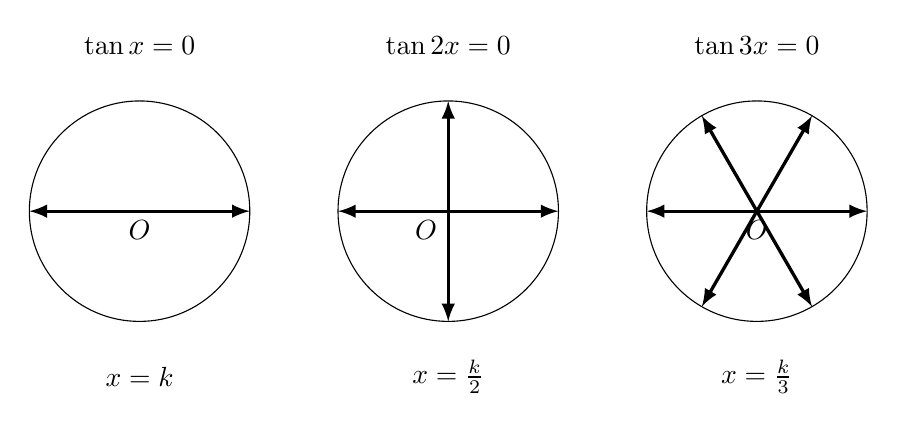
\begin{tikzpicture}[>=latex, scale=1.4]
\begin{scope}
    \draw (0,0) circle (1);
    \draw[<->, very thick] (0:1)--(180:1);
    \node at (0,0)[below]{$O$};
\node at (0,1.5){$\tan x=0$};
\node at (0,-1.5){$x=k\uppi$};
\end{scope}
\begin{scope}[xshift=2.8cm]
    \draw (0,0) circle (1);
    \draw[<->, very thick] (0:1)--(180:1);
    \draw[<->, very thick] (90:1)--(-90:1);
    \node at (-.2,0)[below]{$O$};
\node at (0,1.5){$\tan 2x=0$};
\node at (0,-1.5){$x=\frac{k\uppi}{2}$};
\end{scope}
\begin{scope}[xshift=5.6cm]
    \draw (0,0) circle (1);
    \draw[<->, very thick] (0:1)--(180:1);
    \draw[<->, very thick] (60:1)--(180+60:1);
    \draw[<->, very thick] (120:1)--(-60:1);
    \node at (0,0)[below]{$O$};
\node at (0,1.5){$\tan 3x=0$};
\node at (0,-1.5){$x=\frac{k\uppi}{3}$};
\end{scope}
\end{tikzpicture} 
    \caption{}
\end{figure}

$\because\quad \tan x=0$的解$x=k\uppi=3k\cdot \frac{\uppi}{3}\in \{x|tan 3x=0\}=\left\{x\big| x=k\cdot \frac{\uppi}{3}\right\}$

又$\tan 2x=0$的解$x=k\cdot \frac{\uppi}{2}$
中,当$k=2n+1$时,使$\tan x$没有确定
值,必须舍去;又当$k=2n$时,
\[x=n\uppi=3n\cdot \frac{\uppi}{3}\in\left\{x\big|x=k\cdot \frac{\uppi}{3}\right\}=\{x|\tan 3x=0\}\]
因此,所求方程的解集是
$\left\{x\big|x=k\cdot \frac{\uppi}{3},\quad k\in\mathbb{Z}\right\}$
\end{solution}

\begin{example}
    解方程
$\sin x+\tan x=\sec x-\cos x$
\end{example}

\begin{solution}
两边同乘以$\cos x$, 得到
$\sin x\cos x+\sin x=1-\cos^2x$
移项,提取公因式得
\[\sin x(\cos x +1-\sin x)=0\]
由此得
\[\sin x=0\quad  \text{或}\quad \cos x+1-\sin x=0\]

由 $\sin x=0$, 得 $x=k\uppi$。 

由 $\sin x-\cos x=1$,变形为 $\sin x-\sin(90^{\circ}-x)=1$,即:
\[2\cos45^{\circ} sin\left(x-\frac{\uppi}{4}\right)=1\]
即 $\sin\left(x-\frac{\uppi}{4}\right)=\frac{\sqrt{2}}{2}$

由此得:
\[x-\frac{\uppi}{4}=\frac{\uppi}{4}+2k\uppi\quad  \text{或}\quad x-\frac{\uppi}{4}=\frac{3\uppi}{4}+2k\uppi\]
即
\[x=\frac{\uppi}{2}+2k\uppi\quad  \text{或}\quad x=(2k+1)\uppi\]
这样,我们由已知方程得到 3 组解:
\begin{align}
    x&=k\uppi\\
    x&=\frac{\uppi}{2}+2k\uppi\\
    x&=(2k+1)\uppi
\end{align}
因为$\{x|x=(2k+1)\uppi\}\subset \{x|x=k\uppi\}$,又$x=\frac{\uppi}{2}+2k\uppi$使$\cos x=0$,因此对于$x$的这些值,原方
程中的函数$\tan x$及$\sec x$无意义,这就是说$x=\frac{\uppi}{2}+2k\uppi$是增
根,必须舍去,所以原方程的解集是$\{x|x=k\uppi,\; k\in\mathbb{Z}\}$。
\end{solution}

\begin{example}
    解方程$\sin7x=\sin5x$
\end{example}

\begin{solution}    
\emph{解法1:}移项,得$\sin7x-\sin5x=0$,利用和差化积公式得
\[2\cos6x\sin x=0\]
由此得
\[\cos6x=0\quad  \text{或}\quad \sin x=0\]
由$\cos6x=0$,得:
\[\begin{split}
    6x&=\frac{\uppi}{2}+k\uppi\\
    x&=\frac{\uppi}{12}+k\cdot \frac{\uppi}{6}
\end{split} \]
由$\sin x=0$,得:$x=k\uppi$。
    
所求方程的解集是
\[\left\{x\big|x=\frac{\uppi}{12}+k\cdot \frac{\uppi}{6}\right\}\cup\left\{x\big|x=k\uppi\right\} \]
    
\emph{解法2:} 利用二角正弦相等条件有
\[7x=5x+2k\uppi \quad \text{或}\quad 7x=\uppi -5x+2k\uppi \]

由$7x=5x+2k\uppi$得 $2x=2k\uppi$,因此:$x=k\uppi$。

由$7x=\uppi -5x+2k\uppi$得
$12x=\uppi +2k\uppi$, 因此:$x=\frac{\uppi}{12}+k\cdot \frac{\uppi}{6}$

$\therefore\quad $方程的解集是
\[\left\{x\big|x=k\uppi\right\}\cup\left\{x\big|x=\frac{\uppi}{12}+k\cdot \frac{\uppi}{6}\right\} \]

我们得到与第一种解法相同的结果。
\end{solution}

\subsubsection{$a\sin x +b\cos x=c$型的方程}

\paragraph{第一种方法} 引入辅助角$\varphi$,让方程的两端除以$\sqrt{a^2+b^2}$, 得到
\[\frac{a}{\sqrt{a^{2}+b^{2}}} \sin x+\frac{b}{\sqrt{a^{2}+b^{2}}} \cos x=\frac{c}{\sqrt{a^{2}+b^{2}}}\]
令$\cos \varphi=\frac{a}{\sqrt{a^{2}+b^{2}}}, \quad \sin \varphi=\frac{b}{\sqrt{a^{2}+b^{2}}}$,
由点 $(a, b)$ 所在的象限定出角 $\varphi$ 是第几象限角, 可由 
$\tan \varphi=\frac{b}{a}$ 求出$\varphi$的值, 于是原方程可写成
\[\sin x \cos \varphi+\cos x \sin \varphi=\frac{c}{\sqrt{a^{2}+b^{2}}}\]
即 $\sin (x+\varphi)=\frac{c}{\sqrt{a^{2}+b^{2}}}$

解出 
\begin{equation}
    x+\varphi=2 k \uppi+\arcsin \frac{c}{\sqrt{a^{2}+b^{2}}}
\end{equation}
或
\begin{equation}
    x+\varphi=2 k \uppi+\uppi-\arcsin \frac{c}{\sqrt{a^{2}+b^{2}}}
\end{equation}
由此得到
\[x=2 k \uppi+\arcsin \frac{c}{\sqrt{a^{2}+b^{2}}}-\varphi\]
或
\[x=(2 k+1) \uppi-\arcsin \frac{c}{\sqrt{a^{2}+b^{2}}}-\varphi\]

讨论:原方程有解的必要且充分条件是 $\left| \dfrac{c}{\sqrt{a^{2}+b^{2}}}\right|\leqslant 1$,即 $\dfrac{c^2}{a^2+b^2}\leqslant 1$,由此得到
$a^2+b^2\geqslant c^2$。

\begin{example}
  解方程 $-\sqrt{3}\sin x+\cos x=1$
\end{example}

\begin{solution}
原方程两边除以 $\sqrt{(-\sqrt{3})^2+1}=2$,得到
\[-\frac{\sqrt{3}}{2}\sin x+\frac{1}{2}\cos x=\frac{1}{2}\]
令 $\cos\varphi=-\frac{\sqrt{3}}{2}<0,\quad \sin\varphi=\frac{1}{2}>0$,则角 $\varphi$ 是第一象限角,
\[\varphi=\arccos\left(-\frac{\sqrt{3}}{2}\right)=\uppi-\arccos\frac{\sqrt{3}}{2}=\uppi-\frac{\uppi}{6}=\frac{5\uppi}{6}\]
于是,原方程可写成
\[\sin x\cos\frac{5\uppi}{6}+\cos x\sin \frac{5\uppi}{6}=\frac{1}{2}\]
即:$\sin\left(x+\frac{5\uppi}{6}\right)=\frac{1}{2}$。

$\therefore\quad x+\frac{5\uppi}{6}=2k\uppi+\frac{\uppi}{6}\quad \text{或}\quad x+\frac{5\uppi}{6}=2k\uppi+\left(\uppi-\frac{\uppi}{6}\right)$

由此:$x=2k\uppi-\frac{2\uppi}{3}\quad \text{或}\quad x=2k\uppi$。

$\therefore\quad $原方程的解集是
\[\left\{x\big|x=2k\uppi-\frac{2\uppi}{3}\right\}\cup \left\{x\big|x=2k\uppi\right\}\]
\end{solution}

\begin{example}
    解方程$2\sin x-3\cos x =\sqrt{13}$
\end{example}

\begin{solution}
方程两边除以$\sqrt{2^2+(-3)^2}=\sqrt{13}$, 得到
\[\frac{2}{\sqrt{13}}\sin x+\frac{(-3)}{\sqrt{13}}\cos x=1\]
令$\cos\varphi=\frac{2}{\sqrt{13}}>0,\quad \sin\varphi=\frac{-3}{\sqrt{13}}<0$则角$\varphi$是第四象限角,且由$\tan \varphi=-\frac{3}{2}=-1.5$, 查表得出
$\varphi=\arctan (-1.5)\approx -56^{\circ}18'$, 于是原方程可写成
\[\sin x\cos(-56^{\circ}18')+\cos x\sin(-56^{\circ}18')=1\]
即:
$\sin(x-56^{\circ}18')=1$,由此:
\[\begin{split}
   x- 56^{\circ}18'&=k\cdot 360^{\circ}+90^{\circ}\\
x&=k\cdot 360^{\circ}+146^{\circ}18'
\end{split}\]

$\therefore\quad $原方程的解集是$\{x\big|x=k\cdot 360^{\circ}+146^{\circ}18'\}$。
\end{solution}

\paragraph{第二种方法} 
利用$\tan\frac{x}{2}$表$\sin x$和$\cos x$的公式(“万能
公式”),
\[\sin x=\frac{2\tan\frac{x}{2}}{1+\tan^2\frac{x}{2}},\qquad \cos x=\frac{1-\tan^2\frac{x}{2}}{1+\tan^2\frac{x}{2}}\]

例如,$-\sqrt{3}\sin x+\cos x=1 $,可写成
\[\frac{-\sqrt{3}\cdot 2\tan\frac{x}{2}}{1+\tan^2\frac{x}{2}}+\frac{1-\tan^2\frac{x}{2}}{1+\tan^2\frac{x}{2}}=1\]
化简得
\[\begin{split}
    2\tan^2\frac{x}{2}+2\sqrt{3}\tan\frac{x}{2}&=0\\
    2\tan\frac{x}{2}\left(\tan\frac{x}{2}+\sqrt{3}\right)&=0
\end{split} 
   \]
$\therefore\quad \tan\frac{x}{2}=0\quad \text{或}\quad \tan\frac{x}{2}+\sqrt{3}=0$

由$\tan\frac{x}{2}=0$得$\frac{x}{2}=k\uppi$,\quad $\therefore\quad x=2k\uppi$

由$\tan\frac{x}{2}=-\sqrt{3}$得$\frac{x}{2}=k\uppi+\arctan(-\sqrt{3})$

$\therefore\quad x=2k\uppi+2\left(-\frac{\uppi}{3}\right)=2k\uppi-\frac{2\uppi}{3}$

因为原方程不含使$\tan\frac{x}{2}$
失去意义的解$x=(2k+1)\uppi$, 所以用万能公式进行代换不会丢根。

$\therefore\quad $原方程的解集是
\[\left\{x\big|x=2k\uppi-\frac{2}{3}\uppi\right\}\cup \left\{x\big|x=2k\uppi\right\}\]
所得结果与例9.36第一种解法相同。

\paragraph{第三种方法} 化为$\sin\frac{x}{2}$和$\cos \frac{x}{2}$
的二次齐次方程,例
如$-\sqrt{3}\sin x+\cos x=1$, 可写成
\[-2\sqrt{3}\sin\frac{x}{2}\cos \frac{x}{2}+\cos^2\frac{x}{2}-\sin^2\frac{x}{2}=\cos^2\frac{x}{2}+\sin^2\frac{x}{2}\]
化简为
\[\begin{split}
    -2\sqrt{3}\sin\frac{x}{2}\cos\frac{x}{2}-2\sin^2\frac{x}{2}&=0\\
    -2\sin\frac{x}{2}\left(\sqrt{3}\cos\frac{x}{2}+\sin\frac{x}{2}\right)&=0
\end{split}\]
由$\sin\frac{x}{2}=0$, 得到
$\frac{x}{2}=k\uppi ,\quad \therefore\quad x=2k\uppi $

由$\sqrt{3}\cos\frac{x}{2}+\sin \frac{x}{2}=0$, 两边除以$\cos\frac{x}{2}$
得:
\[\begin{split}
    \sqrt{3}+\tan\frac{x}{2} &=0\\
    \tan\frac{x}{2}&=-\sqrt{3}\\
    \frac{x}{2}&=k\uppi-\frac{\uppi}{3}\\
    x&=2k\uppi-\frac{2\uppi}{3}
\end{split}\]
$\therefore\quad $原方程的解集是
\[\left\{x\big|x=2k\uppi\right\}\cup \left\{x\big|x=2k\uppi-\frac{2}{3}\uppi\right\}\]
所得结果与例9.36第一种解法相同。

\section{三角不等式的解法}
\begin{Theorem}{定理}
  若函数 $f(x)$ 在 $[a,b]$ 上到处连续且对于任何一个 $x\in (a,b)$,$f(x)\ne 0$,则 $f(x)$ 在 $(a,b)$ 上保持相同符号。
\end{Theorem}

\begin{proof}
用反证法,假设 $f(x)$ 在 $(a,b)$ 内的值有相异的符号,即存在 $x_1$ 和 $x_2$ 满足 $a<x_1<x_2<b$ 且使 $f(x_1)f(x_2)<0$,于是根据连续函数中间值定理,必存在一个介于 $x_1$ 和 $x_2$ 之间的常数 $c$, 使得 $f(c)=0$。这和已知条件:对于任何一个 $x\in
(a,b)$,$f(x)\ne 0$ 矛盾,因此,$f(x)$ 在$ (a,b)$ 内保持相同符号。
\end{proof}

我们举例说明如何应用这个定理解不等式。

\begin{example}
  解不等式 $\sin x>a$
\end{example}

\begin{solution}
移项,化为 $\sin x-a>0$

设 $f(x)=\sin x-a$,$f(x)$ 是周期等于 $2\uppi$ 的函数,先讨论在长度等于一个周期的区间 $\left[-\dfrac{\uppi}{2}, \dfrac{3\uppi}{2}\right]$ 内的 $f(x)$ 的符号:
\begin{enumerate}
  \item 若 $|a|\leqslant 1$, 求 $f(x)$ 在 $\left[-\dfrac{\uppi}{2}, \dfrac{3\uppi}{2}\right]$ 内的零点。$\sin x=a$在$\left[-\dfrac{\uppi}{2}, \dfrac{3\uppi}{2}\right]$ 内的解是
  \[x_1=\arcsin a \quad \text{和}\quad x_2=\uppi-\arcsin a\]
  把解的终边画在单位圆上,如\cref{fig:unit_circle_solution1} 且由\cref{fig:unit_circle_solution1} 看出:
  \begin{figure}
    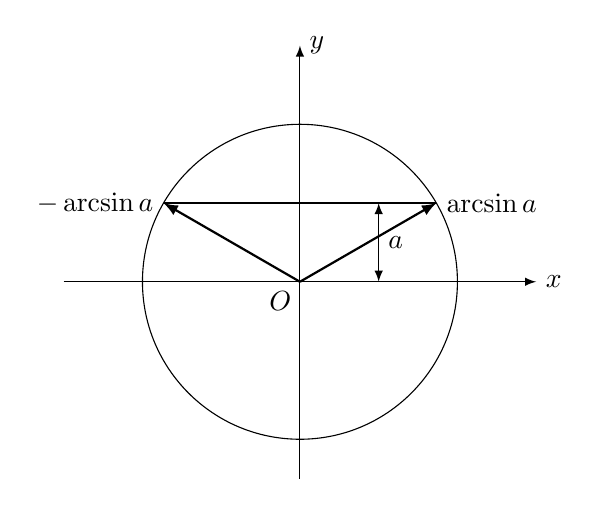
\begin{tikzpicture}[>=latex]
      \draw[->] (-3,0)--(3,0)node[right]{$x$};
      \draw[->] (0,-2.5)--(0,3)node[right]{$y$};
      \node at (-.25,-.25){$O$};
      \draw (0,0) circle(2);
      \draw[thick,->] (0,0)--(30:2)node[right]{$\arcsin a$};
      \draw[thick,->] (0,0)--(150:2)node[left]{$\uppi-\arcsin a$};
      \draw (30:2)--(150:2);
      \draw[<->] (1,0)--node[right]{$a$}(1,1);
    \end{tikzpicture}
    \caption{}\label{fig:unit_circle_solution1}
  \end{figure}

  当 $\arcsin a<x<\uppi-\arcsin a$ 时,$f(x)=\sin x-a>0$ 成立;

  当 $-\dfrac{\uppi}{2}<x<\arcsin a$ 或 $\uppi-\arcsin a<x<\dfrac{3\uppi}{2}$ 时,$f(x)=\sin x-a<0$ 成立,因此,在 $|a|\leqslant 1$ 的场合,$\sin x>a$ 在 $\left[-\dfrac{\uppi}{2}, \dfrac{3\uppi}{2}\right]$ 内的解满足条件:
  \[\arcsin a<x<\uppi-\arcsin a\]
  由于 $f(x)=\sin x-a$ 是周期等于 $2\uppi$ 的函数,因此 $\sin x>a$ 的一切解满足条件:
  \[2k\uppi+\arcsin a<x<(2k+1)\uppi-\arcsin a,\quad k\in\mathbb{Z}\]
  \item 若 $a>1$, 则对于任何 $x\in\mathbb{R}$,有 $f(x)=\sin x-a<0$,因此,不等式 $\sin x>a$ 没有解。
  \item 若 $a<-1$,则对于任何 $x\in\mathbb{R}$,有 $f(x)=\sin x-a>0$,因此,不等式 $\sin x>a$ 的解集是实数集 $\mathbb{R}$。
\end{enumerate}

总之:
\begin{enumerate}
  \item 当 $|a|\leqslant 1$ 时,所求不等式的解集是
  \[\{x|2k\uppi+\arcsin a<x<(2k+1)\uppi-\arcsin a\}\]
  \item 当 $a>1$ 时,所求不等式的解集是空集 $\emptyset$;
  \item 当 $a<-1$ 时,所求不等式的解集是实数集 $\mathbb{R}$。
\end{enumerate}
\end{solution}

\begin{example}
  解不等式 $\cos x<a$
\end{example}

\begin{solution}
移项,化为 $\cos x-a<0$

设 $f(x)=\cos x-a$,$f(x)$ 是周期等于 $2\uppi$ 的函数,先讨论在长度等于一个周期的区间 $[-\uppi,\uppi]$ 内的 $f(x)$ 的符号:
\begin{enumerate}
  \item 若 $|a|\leqslant 1$,$f(x)=\cos x-a$ 在 $[-\uppi,\uppi]$ 内的解是
  \[x_1=\arccos a\quad \text{和}\quad x_2=-\arccos a\]
  把解的终边画在单位圆上,如\cref{fig:unit_circle_solution2} 且由\cref{fig:unit_circle_solution2} 容易
看出:
  \begin{figure}
    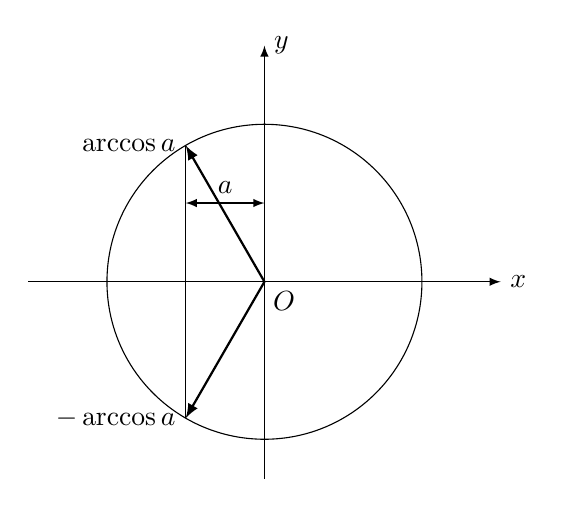
\begin{tikzpicture}[>=latex]
      \draw[->] (-3,0)--(3,0)node[right]{$x$};
      \draw[->] (0,-2.5)--(0,3)node[right]{$y$};
      \node at (.25,-.25){$O$};
      \draw (0,0) circle(2);
      \draw[thick,->] (0,0)--(120:2)node[left]{$\arccos a$};
      \draw[thick,->] (0,0)--(-120:2)node[left]{$-\arccos a$};
      \draw (120:2)--(-120:2);
      \draw[<->] (0,1)--node[above]{$a$}(-1,1);
    \end{tikzpicture}
    \caption{}\label{fig:unit_circle_solution2}
  \end{figure}

当 $\arccos a<x<\uppi$ 或 $-\uppi <x<-\arccos a$ 时,$f(x)=\cos x-a<0$ 成立,而且仅在此时成立,又因为 $f(x)=\cos x-a$的周期是 $2\uppi$,所以,$\cos x<a$ 的一切解,满足
\begin{equation}
  \label{eq:solution_cos_negative}
   2k\uppi +\arccos a<x<(2k+1)\uppi  
\end{equation}
或
\begin{equation}
  \label{eq:solution_cos_positive}
    (2k-1)\uppi <x<2k\uppi -\arccos a
\end{equation}
又\cref{eq:solution_cos_positive} 也可以写成
\begin{equation}
  \label{eq:solution_cos_positive2}
    (2k+1)\uppi <x<(2k+2)\uppi -\arccos a
\end{equation}
再将\cref{eq:solution_cos_negative,eq:solution_cos_positive2} 合并为
\begin{equation}
  \label{eq:solution_cos}
  2k\uppi +\arccos a<x<(2k+2)\uppi -\arccos a
\end{equation} 
因此,在 $|a|\leqslant 1$ 的场合,$\cos x<a$ 的一切解满足 \eqref{eq:solution_cos}。

\item 若 $a>1$,则对于任何 $x\in\mathbb{R}$,有$f(x)=\cos x-a<0$ 成立,因此,不等式 $\cos x<a$ 的解集是实数集 $\mathbb{R}$。
\item 若$a<-1$,则对于任何 $x\in\mathbb{R}$,有 $f(x)=\cos x-a>0$ 成立,因此,不等式 $\cos x<a$ 没有解。
\end{enumerate}

总之,
\begin{enumerate}
  \item 当 $|a|\leqslant 1$ 时,所求不等式的解集是
  \[\{x|2k\uppi  +\arccos a<x<(2k+2)\uppi -\arccos a\}\]
  \item 当 $a>1$ 时,所求不等式的解集是实数集 $\mathbb{R}$。
  \item 当 $a<-1$ 时,所求不等式的解集是空集 $\emptyset$。
\end{enumerate}
\end{solution}


\begin{example}
  解不等式 $2\cos^2 2x<1$
\end{example}

\begin{solution}
移项,化简为 $\cos4x<0$。设 $f(x)=\cos4x$,它是周期等于 $\dfrac{2\uppi}{4}=\dfrac{\uppi}{2}$ 的函数。

$f(x)=\cos4x$ 在 $\left[0,\dfrac{\uppi}{2}\right]$ 内的零点为 $\dfrac{\uppi}{8}$,$\dfrac{3\uppi}{8}$。

显然,当 $0\leqslant x<\dfrac{\uppi}{8}$ 时,$f(x)=\cos4x>0$;当 $\dfrac{\uppi}{8}<x<\dfrac{3\uppi}{8}$ 时,$f(x)=\cos4x<0$;当 $\dfrac{3\uppi}{8}<x\leqslant \dfrac{\uppi}{2}$ 时,$f(x)=\cos4x>0$。

$\therefore\quad \cos4x<0$ 在 $\left[0,\dfrac{\uppi}{2}\right]$ 内的部分解满足条件:$\dfrac{\uppi}{8}<x<\dfrac{3\uppi}{8}$

又 $f(x)$ 的周期是 $\dfrac{\uppi}{2}$。

$\therefore\quad \cos4x<0$ 的一切解满足条件
\[\frac{\uppi}{8}+n\cdot\frac{\uppi}{2}<x<\frac{3\uppi}{8}+n\cdot\frac{\uppi}{2}\qquad (n\in\mathbb{Z})\]
$\therefore\quad 2\cos^2 2x<1$ 的解集是
\[\left\{x\Big| \frac{\uppi}{8}+n\cdot\frac{\uppi}{2}<x<\frac{3\uppi}{8}+n\cdot\frac{\uppi}{2}\right\}\]
\end{solution}


\begin{example}
  解不等式 $\dfrac{\cos2x+\cos x-1}{\cos2x}>2,\quad (0<x<2\uppi)$
\end{example}

\begin{solution}
移项,并将 $\cos2x=2\cos^2x-1$ 代入得
\[\frac{\cos x(1-2\cos x)}{2\cos^2x-1}>0\] 
因为原不等式的解使 $\cos2x\ne 0$(即 $2\cos^2x-1\ne 0$),两边乘以 $(2\cos^2x-1)^2$,得到同解不等式
\[\cos x(1-2\cos x)(2\cos^2x-1)>0\]
即
\[\left(\cos x+\frac{1}{\sqrt{2}}\right)\cos x\left(\cos x-\frac{1}{2}\right)\left(\cos x-\frac{1}{\sqrt{2}}\right)<0\]
上面不等式右端的函数式 $f(x)$ 的零点依大小排列是 $-\dfrac{1}{\sqrt{2}},\; 0,\; \dfrac{1}{2},\; \dfrac{1}{\sqrt{2}}$。由此得知,仅当
\begin{equation}
  \label{eq:solution_quadrant2}
  -\frac{1}{\sqrt{2}}<\cos x<0
\end{equation}
或
\begin{equation}
  \label{eq:solution_quadrant1}
  \frac{1}{2}<\cos x<\frac{1}{\sqrt{2}}
\end{equation}
时,$f(x)=\cos x(1-2\cos x)(2\cos^2x-1)<0$。

由于 $\cos x$ 在区间 $[0,\uppi]$ 内是递减的,在区间 $[\uppi,2\uppi]$ 内
是递增的,所以由不等式 \eqref{eq:solution_quadrant2}, 得(\cref{fig:solution_negative}):
\[\frac{\uppi}{2}<x<\frac{3\uppi}{4},\qquad \frac{5\uppi}{4}<x<\frac{3\uppi}{2}\]
由不等式 \eqref{eq:solution_quadrant1}, 得(\cref{fig:solution_positive}):
\[\frac{\uppi}{4}<x<\frac{\uppi}{3},\qquad \frac{5\uppi}{3}<x<\frac{7\uppi}{4}\]
因此,原不等式在区间 $0<x<2\uppi$ 内的解集是
\[\left\{x\Big|\frac{\uppi}{4}<x<\frac{\uppi}{3} \right\}\bigcup\left\{x\Big|\frac{\uppi}{2}<x<\frac{3\uppi}{4} \right\}\bigcup\left\{x\Big|\frac{5\uppi}{4}<x<\frac{3\uppi}{2} \right\}\bigcup\left\{x\Big|\frac{5\uppi}{3}<x<\frac{7\uppi}{4} \right\}\]
\end{solution}

\begin{figure}
  \begin{minipage}[t]{0.48\textwidth}
    \centering
    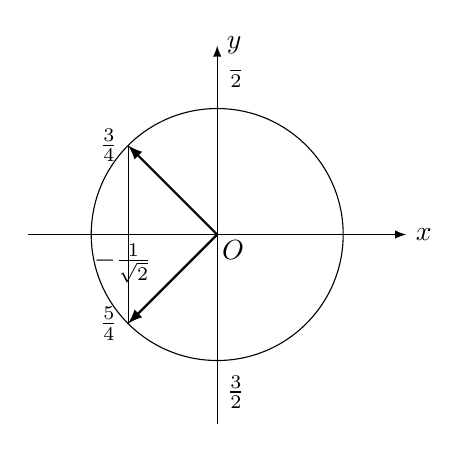
\begin{tikzpicture}[>=latex, scale=.8]
      \draw[->] (-3,0)--(3,0)node[right]{$x$};
      \draw[->] (0,-3)--(0,3)node[right]{$y$};
      \node at (.25,-.25){$O$};
      \draw (0,0) circle(2);
      \draw[thick,->] (0,0)--(135:2)node[left]{$\frac{3\uppi}{4}$};
      \draw[thick,->] (0,0)--(-135:2)node[left]{$\frac{5\uppi}{4}$};
      \draw (135:2)--(-135:2);
      \node at (0,2.5)[right]{$\frac{\uppi}{2}$};
      \node at (0,-2.5)[right]{$\frac{3\uppi}{2}$};
      \node at (-1.5,0)[below]{$-\frac{1}{\sqrt{2}}$};
    \end{tikzpicture}
    \caption{}\label{fig:solution_negative}
  \end{minipage}
  \begin{minipage}[t]{0.48\textwidth}
    \centering
    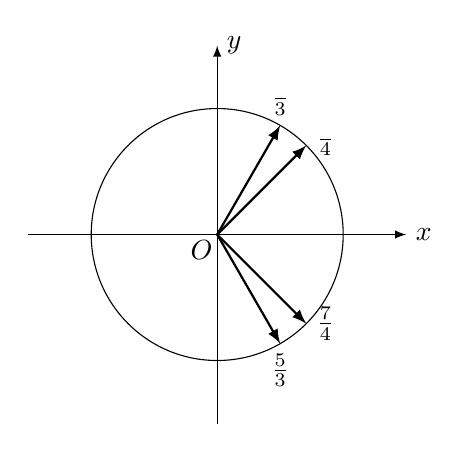
\begin{tikzpicture}[>=latex, scale=.8]
      \draw[->] (-3,0)--(3,0)node[right]{$x$};
      \draw[->] (0,-3)--(0,3)node[right]{$y$};
      \node at (-.25,-.25){$O$};
      \draw (0,0) circle(2);
      \draw[thick,->] (0,0)--(45:2)node[right]{$\frac{\uppi}{4}$};
      \draw[thick,->] (0,0)--(-45:2)node[right]{$\frac{7\uppi}{4}$};
      \draw[thick,->] (0,0)--(60:2)node[above]{$\frac{\uppi}{3}$};
      \draw[thick,->] (0,0)--(-60:2)node[below]{$\frac{5\uppi}{3}$};
    \end{tikzpicture}
    \caption{}\label{fig:solution_positive}
  \end{minipage}
\end{figure}

\begin{Exercise}
\begin{question}
  \item 解下列方程:
  \begin{tasks}(2)
    \task $\sin x=1$
    \task $\sin x=0$
    \task $\cos x=0$
    \task $\cos x=1$
    \task $\cot x=0$
    \task $\sin x=\dfrac{\sqrt{3}}{2}$
    \task $\sin\left(x+\dfrac{\uppi}{6}\right)=-\dfrac{1}{2}$
    \task* $\cos\left(x+\dfrac{\uppi}{6}\right)=\dfrac{1}{2}$
    \task $\tan \left(x-\dfrac{\uppi}{3}\right)=-\sqrt{3}$
    \task $\tan \left(x+\dfrac{\uppi}{4}\right)=-1$
    \task $\cot \dfrac{2x}{3}-1=0$
    \task $\cos\left(x+\dfrac{\uppi}{4}\right)=-\dfrac{\sqrt{3}}{2}$
  \end{tasks}
  \item 解下列各方程(用反三角函数符号表示各方程的解):
  \begin{tasks}(2)
    \task $\sin2x=0.7$
    \task $\tan 3x=3$
    \task $\cot (2x-1)=\sqrt{2}$
    \task $\cos\dfrac{\alpha}{2}=\dfrac{1}{5}$
    \task $\cot \dfrac{x}{4}=\dfrac{1}{4}$
    \task $\sin\left(\alpha+\dfrac{\uppi}{3}\right)=0.1$
    \task $\cos\left(2x-\dfrac{\uppi}{10}\right)=0.85$
    \task $\tan \left(\dfrac{x}{2}+\dfrac{\uppi}{5}\right)=\dfrac{1}{8}$
  \end{tasks}
  \item 解下列各方程:
  \begin{tasks}(2)
    \task $2 \sin \dfrac{x+1}{4}+1=0$
    \task $4 \sin ^{2} 4 x-3=0$
    \task $2 \sin ^{2} x-3 \sin x+1=0$
    \task $\tan ^{2} 3 x=2 \tan  3 x$
    \task! $\cot^{2}\left(\dfrac{x}{2}-\dfrac{\uppi}{8}\right)+3 \cot\left(\dfrac{x}{2}-\dfrac{\uppi}{8}\right)-4=0$
    \task  $4 \cos ^{2} x+\sin x=1$
    \task  $\tan  x+5 \cot x=6$
    \task  $2 \cot 3 x+\tan  3 x+3=0$
  \end{tasks}
  \item $a,b,c$ 满足什么条件,方程 $a\sin^2 x+b\cos^2 x=c$ 有解。
  \item 解下列各方程:
  \begin{tasks}(2)
    \task  $\sin x(1+2 \cos x)=0$
    \task  $\sin 2 x \cos 3 x=0$
    \task  $\cos \left(2 x+\dfrac{\uppi}{3}\right) \sin \left(3 x-\dfrac{\uppi}{3}\right)=0$
    \task  $\cos 5 x(1+\cos 2 x)=0$
    \task! $\cot x-\cos x=1-\sin x$
    \task! $1+\sin x \cos 3 x+\sin x+\cos 3 x=0$
    \task  $\dfrac{\cos x}{1+\sin x}=2-\tan x$
    \task  $\sin 3 x \cdot \cot x=0$
  \end{tasks} 
  \item 解下列各方程:
  \begin{tasks}(2)
    \task   $\sin 3 x=\cos 3 x$
    \task   $\sin ^{2} 3 x=3 \cos ^{2} 3 x$
    \task!  $ 5 \cos x+2 \sin x=5 \cos x \cos 2 x+2 \sin x \cos 2 x$   
    \task!  $\sin x \tan x+\cos x \cdot \cot x=\sin x+\cos x$
    \task!  $\sin ^{2} x+5 \sin x \cos x+4 \cos ^{2} x=0$
    \task! $3 \sin ^{2} x-7 \sin x \cos x+6 \cos ^{2} x=1$
    \task!  $\dfrac{\sin x+2 \cos x}{\sin x-2 \cos x}=3$
    \task!  $\dfrac{2 \sin ^{2} x-4 \cos ^{2} x}{\sin ^{2} x+3 \sin x \cos x+6 \cos ^{2} x}=1$
  \end{tasks}
  \item $a, b$ 满足什么条件, 方程 $\dfrac{a^{2} \sin x^{2}+b \cos x^{2}}{b^{2} \sin ^{2} x+a \cos x}=1$ 有解。
  \item 解下列各方程:
  \begin{tasks}(2)
    \task  $\sin 3 x \cos x=\cos 3 x \sin x$
    \task  $\cos 7 x \cos 3 x=\cos 4 x$
    \task! $\sin \left(\dfrac{\uppi}{2}-x\right) \cos 2 x+\sin (2 x-\uppi) \sin x=0$
    \task! $\sin \dfrac{3 \uppi-x}{2} \cos \left(\dfrac{\uppi}{2}-3 x\right) =\cos (3 x-\uppi) \cos \dfrac{3 \uppi+x}{2}$
    \task  $\tan x\cdot \tan\left(3x-\dfrac{\uppi}{4}\right)=1$
    \task  $\sin x\cos x=\dfrac{1}{4}$
    \task  $\sin(\ang{34}+x)\sin(\ang{56}-x)=\dfrac{\sqrt{2}}{4}$
    \task  $\cos^4x-\sin^4x=1$
    \task! $\cos ^{2}\left(x+\ang{30}\right)-\sin ^{2}\left(x+\ang{30}\right)=\dfrac{1}{2}$
    \task! $\sin \left(x+\dfrac{\uppi}{10}\right) \sin \left(\dfrac{2 \uppi}{5}-x\right)=\dfrac{\sqrt{2}}{4}$
    \task  $\sin \left(x+\dfrac{\uppi}{6}\right)=2 \cos x$
    \task  $1-\tan^{2} x=2 \tan x \tan 2 x$
    \task  $2 \cos 2 x=7 \sin x $
    \task  $\sin 2 x+\sqrt{2} \sin x=0$
    \task  $2 \sin ^{2} x+\sin ^{2} 2 x=2$
    \task  $\dfrac{\cos 2 x}{\cos x-\sin x}=0$
    \task  $\sin 4 x=2 \cos ^{2} x-1 $
    \task  $\sin x \cos x \cos 2 x=\dfrac{1}{8}$
    \task  $\cot x-\tan x=\tan 2 x$
    \task  $2-\sin \dfrac{x}{2}=2 \cos \dfrac{x}{2}$
  \end{tasks}
  \item 解下列各方程:
  \begin{tasks}(2)
    \task  $\sin 2 x=\sin 3 x$
    \task  $\cos \left(2 x+\ang{15}\right)=\cos \left(4 x-\ang{15}\right)$
    \task  $\tan\left(\dfrac{x}{2}+\ang{30}\right)=\tan\left(2 x+\ang{60}\right)$
    \task  $\cos 3 x=\sin \left(x-\dfrac{\uppi}{6}\right)$,
    \task  $\tan\left(\dfrac{\uppi}{8}-x\right)=\cot\left(\dfrac{\uppi}{4}+3 x\right)$
    \task  $\sin 2 x=-\sin \dfrac{x}{2}$
    \task  $\tan 3 x+\cot \dfrac{x}{3}=0$
    \task  $\sin 3 x+\dfrac{\sqrt{3}}{2} \sin 2 x=\dfrac{1}{2} \cos 2 x$
    \task  $\cos x-\sin x=1$
    \task  $2 \cos \left(x+\ang{20}\right) \cos x=\cos \ang{40} $
    \task  $\sin x+\cos x=2 \sqrt{2} \sin x \cos x$
    \task  $\sin 3 x \cos x=\sin 7 x \cos 5 x$
    \task! $\cos \left(2 x+\ang{15}\right)+\cos \left(2 x-\ang{15}\right)=\dfrac{1}{2}$
    \task!  $\sin \left(2 x+\dfrac{\uppi}{18}\right) \cos \left(2 x-\dfrac{\uppi}{9}\right)=-\dfrac{1}{4}$
    \task! $\sin \left(x+\ang{15}\right) \sin \left(x-\ang{30}\right)=$ $\sin \left(\ang{50}+x\right) \cos \left(\ang{85}-x\right)$
  \end{tasks}
  \item 解下列各方程:
  \begin{tasks}(2)
    \task $\cos 7 x+\cos x=\cos 4 x$
    \task $\tan x+\tan 2 x=\sin 3 x \cos x$
    \task $\cos 8 x+\cos 6 x=\sqrt{3} \cos x$
    \task $1-\cos 2 x=4 \sin x$
    \task $\sin x+\sin 2x+ \sin 3x= 0$
    \task $\cos x+\cos2x-\cos3x=1$
    \task $\sin2 x+2\sin x=\sin\dfrac{x}{2}$
    \task $1+\cos2x+\sin x=2\cos^2\dfrac{x}{2}$
    \task $\tan x+\tan 2x=\tan 3x$
  \end{tasks}
  \item 解下列各方程:
  \begin{tasks}(2)
    \task $\sin ^{2}\left(x+10^{\circ}\right)-\sin ^{2} x=\dfrac{1}{2} \sin 20^{\circ}$
    \task $\sin ^{2} x+\sin ^{2} 2 x+\sin ^{2} 3 x=\dfrac{3}{2}$
    \task $\cos ^{2} x+\cos ^{2} 2 x+\cos ^{2} 3 x=1$
    \task $\sin ^{2} 2 x+\sin ^{2} 4 x=\dfrac{3}{2}$
    \task $\sqrt{3} \cos x+\sin x=\sqrt{3} $
    \task $4 \sin x+3 \cos x=2 $
    \task $\sin 3 x+2 \cos 2 x=1 $
    \task! $5 \cos \left(2 x+18^{\circ}\right)-12 \sin \left(2 x+18^{\circ}\right)=13$
    \task! $(4 \sin x-5 \cos x)^{2}-13(4 \sin x-5 \cos x)+42=0$
  \end{tasks}
  \item 解下列方程:
  \begin{tasks}(2)
    \task $\dfrac{1+\tan x}{1-\tan x}=1+\sin 2 x$
    \task $\dfrac{\sin x}{1+\cos x}=2-\cot x$
    \task $\sin 2 x=\cos 2 x-\sin ^{2} x+1$
    \task! $(\cos 5 x+\cos 7 x)^{2}=(\sin 5 x+\sin 7 x)^{2}$
  \end{tasks}
  \item 设关于 $x$ 的方程 $\sin x+\sqrt{3}\cos x+a=0$ 在区间内有相异二解 $\alpha,\beta$。 试求常数 $a$ 的取值范围和 $\tan(\alpha+\beta)$ 的值。
  \item 解下列各方程组:
  \begin{tasks}(2)
    \task $\begin{cases}
        \sin x\sin y=\dfrac{1}{4\sqrt{2}}\\
        \tan x\cdot \tan y=\dfrac{1}{3}
    \end{cases}$
    \task $\begin{cases}
        x+y=\dfrac{\uppi}{4}\\
        \tan x+\tan y=1
    \end{cases}$
    \task $\begin{cases}
        \sin(2x+\sin^2y)=0\\
        x-3\sin^2y=-2
    \end{cases}$
  \end{tasks}
  \item 解下列的不等式:
  \begin{tasks}(2)
    \task $\sin (2 \uppi \cos x)>0$
    \task $\lg \sin x \leqslant 0$
    \task $\cos ^{2} x+7 \sin ^{2} x<8 \sin x \cos x$
    \task $\sin x+\sqrt{3} \cos x>1$
    \task! $2 \cos ^{2}\left(x+30^{\circ}\right)-3 \sin \left(60^{\circ}-x\right)+1>0$
  \end{tasks}
  \item 求下列各函数的定义域:
  \begin{tasks}(2)
    \task $y=\arccos \dfrac{3}{x}$
    \task $y=\arcsin \dfrac{2 x}{1+x^{2}}$
    \task $y=\sqrt{\sin x}$
    \task $y=\sqrt{4 \cos ^{2} 2 x-3}$
  \end{tasks} 
\end{question}
\end{Exercise}